\documentclass[12pt, oneside]{article}   	% use "amsart" instead of "article" for AMSLaTeX format
\usepackage[margin=1.25in]{geometry}
\geometry{a4paper}                   		% ... or a4paper or a5paper or ... 
%\geometry{landscape}                		% Activate for rotated page geometry
%\usepackage[parfill]{parskip}    		% Activate to begin paragraphs with an empty line rather than an indent
\usepackage{graphicx}				% Use pdf, png, jpg, or eps with pdflatex; use eps in DVI mode
								% TeX will automatically convert eps --> pdf in pdflatex		
\usepackage{amsmath}
\usepackage{mathptmx}
\usepackage{mathtools}
\usepackage{amssymb}        % so we can use the 'pretty' empty set
\usepackage{tipa}
\usepackage{graphicx}           % purdy pitchers
\graphicspath{{diagrams/}}
\usepackage{algorithmic}
\usepackage{phonrule}
\usepackage{ragged2e}
\setlength{\RaggedRightParindent}{\parindent}
\usepackage[compact]{titlesec}
\usepackage{titling}
\usepackage{caption}
\usepackage{tikz-qtree}
\usepackage{tikz}
\usetikzlibrary{shapes,snakes}
\usetikzlibrary{automata,positioning,calc}

\tikzset{
	double arrow/.style args={#1 colored by #2 and #3}{
		-stealth,line width=#1,#2, % first arrow
		postaction={draw,-stealth,#3,line width=(#1)/3,
			shorten <=(#1)/3,shorten >=2*(#1)/3}, % second arrow
	}
}

%% Make footnotes endnotes
%\usepackage{endnotes}
%\let\footnote=\endnote
%
%% Move figures and tables to end
%\usepackage[nomarkers,nolists,noheads]{endfloat}

\usepackage{cite}
\usepackage{apacite}
\usepackage[section]{placeins}
\usepackage{subfig}
\usepackage{setspace}

% Reduce in-text citations to 'et al' when there are more than 2 authors
\makeatletter
\usepackage{regexpatch}
\xpatchcmd{\@@cite}{\def\BCA##1##2{{\@BAstyle ##1}}}{\def\BCA##1##2{{\@BAstyle ##2}}}{}{}
\makeatother

\newtheorem{definition}{Definition}

\newenvironment{clump}
{
	\edef\myindent{\the\parindent}
	\noindent\begin{minipage}{\textwidth}
	\setlength\parindent{\myindent}\fussy
}
{
	\end{minipage}
}
\newcommand{\featmat}[1]
{$[$#1$]$}
%{$\begin{bsmallmatrix*}[l]\text{\normalsize #1}\end{bsmallmatrix*}$}
\newcommand{\featmattwo}[2]{$\begin{bsmallmatrix*}[l]\text{\normalsize #1}\\\text{\normalsize #2}\end{bsmallmatrix*}$}


% make the section headings more compact
\titleformat{\section}{\normalsize\bfseries}{\thesection}{1em}{}
\titleformat{\subsection}{\normalsize\itshape}{\thesubsection}{1em}{}

% make title more compact
\pretitle{\vspace*{-3\baselineskip}\begin{center}\bfseries}
	\posttitle{\par\end{center}}
\preauthor{\begin{center}}
	\postauthor{\par\end{center}}
\predate{}
\postdate{\vspace*{-0.15\baselineskip}}

\makeatletter
\def\blfootnote{\gdef\@thefnmark{}\@footnotetext}
\makeatother

\doublespacing

\title{A method for projecting features from observed sets of phonological classes}

\author{
  Connor Mayer \hspace{20pt} Robert Daland
}
\date{\vspace{-4ex}}							% Activate to display a given date or no date

\begin{document}
\RaggedRight
\maketitle

\begin{abstract}
\noindent \textbf{Abstract:} Given a set of phonological features, we can enumerate a set of phonological classes. Here we consider the inverse of this problem: given a set of phonological classes, can we derive a feature system? We show that this is indeed possible, using a collection of algorithms that assign features to a set of input classes and differ in terms of what types of features are permissible. This work bears on theories of both language-specific and universal features, provides testable predictions of the featurizations available to learners, and serves as a useful component in computational models of feature learning.\\
\noindent \textbf{Keywords}: Phonological features, feature learning, underspecification, computational phonology

\blfootnote{* This research was supported by the Social Sciences and Humanities Research Council of Canada Doctoral Award to the first author. Thanks to Bruce Hayes, Tim Hunter, Kie Zuraw, and the members of the UCLA phonology seminar for their feedback and guidance. All mistakes are our own. Supplemental material can be found at https://github.com/connormayer/featurizer.}
\end{abstract}

% LIST OF FIGURES
% TODO: Move figures to end of document...
%	Fig. 1 (done) -- A manner hierarchy class system
%	Fig. 2 (done) -- A vowel inventory and intersectional closure
%	Fig. 3 (done) -- Yield of the privative specification algorithm (to vowel inventory)
% 	Fig. 4 (done) -- Yield of the contrastive underspecification algorithm (to vowel inventory)
%	Fig. 5 (done) -- Class system and featurization yielded by contrastive specification.
%	Fig. 6 (done) -- Class system and featurization yielded by full specification.
%	Fig. 7 (done) -- Big alphabet (contrastive underspecification with privative, binary, and ternary features)
%	Fig. 8 (done) -- Simple class system to illustrate BFS
%	Fig. 9 (done) -- Featurization of simple class system without and with BFS
%	Fig. 10 (done) -- Simple class system to illustrate sibling ordering considerations
%	Fig. 11 (done) -- Featurization of simple class system if siblings are processed in arbitrary order, or simultaneously.
%	Fig. 12 (done) -- Topological plot of the contrastive specification vowel inventory output.
%	Fig. 13 (done) -- Topological plot of the full specification vowel inventory output.

\section{Introduction}
\label{sec:intro}

Features are the substantive building blocks of phonological theory. They represent phonetic qualities of speech sounds, and can be used in isolation or combination to describe individual sounds or classes of sounds \cite<e.g.,>{JakobsonEtAl1952, ChomskyHalle1968, Clements1985}.

The goals of feature theory are to capture the following generalizations. First, segments that have common phonetic properties tend to behave alike, both within and across languages. Features allow such commonalities between sounds to be explicitly represented. For example, the English voiceless non-continuants \{p, t, \textipa{\t{tS}}, k\} are all produced with a complete closure of the oral cavity and no vocal fold vibration, and exactly these segments undergo the process of foot-initial aspiration. The feature notation \featmattwo{--continuant}{--voice} exposes these shared phonetic properties to the phonological grammar, and the processes which might reference them. More generally, the set of obstruents, which may be specified with the feature \featmat{--sonorant}, tends to undergo similar voicing processes across languages (regressive voicing assimilation within obstruent clusters, word-final devoicing, intervocalic and/or postnasal voicing, etc.).

Common behavior among phonetically similar segments also extends diachronically. For example, the Wakashan language Ditidaht underwent a sound change where all nasal consonants became oral \cite{ThompsonThompson1972}. The feature notation \featmat{+nasal} allows the set of sounds that participated in this change to be specified.

Second, sound changes often preserve phonetic qualities of affected sounds, even when the host segment is altered or destroyed. The sub-segmental representation afforded by features allows these changes to be modeled in a principled way. An instance of feature preservation was the fall of the yers in Old Church Slavonic. The front yer (a short, unstressed, high front vowel) deleted in most prosodic positions. However, the preceding consonant typically became palatalized, preserving the high and front articulations even while the vowel segment was deleted \cite{Carlton1991}. 

Finally, feature theory reflects featural economy in the segmental inventory: if a language treats a particular featural contrast as distinctive, it is likely to be exploited widely throughout its inventory. In other words, segment inventories are more symmetric than might be expected if segments were the atoms of representation \cite{Ohala1980, Maddieson1985, SchwartzEtAl1997, Clements2003}.

Classic texts \cite<e.g.,>{ChomskyHalle1968} have assumed phonological features are \textit{universal}: all the sounds in the world's languages can be described by the same finite set of features, which reflect properties of the human vocal tract and perceptual system. According to this view, speakers inherently produce and perceive speech in terms of these features because they are the substantive `atoms' of which segments and higher prosodic constituents are composed. Children represent speech in terms of these atoms, which is why phonological processes operate on the classes they define. Feature theory is manifestly successful in explaining why many common phonological processes involve segments that share relevant phonetic properties.

However, there is evidence that many phonological processes target sets of segments that cannot be singled out by a set of phonetic properties. A canonical example is the \textit{ruki} rule of Sanskrit, in which an underlying /s/ becomes retroflexed when it occurs later in a word than any of \{r, u, k, i\} \cite<e.g.,>{Kiparsky1973, Vennemann1974}. It has been proposed that the \textit{ruki} process originated from the acoustic effects of these segments on neighboring sounds, e.g., a lowering of the noise frequency of a following /s/ \cite{Longerich1998}. However, no conventional feature system can pick out all four of these segments to the exclusion of others. A more recent example is given by \citeA{Gallagher2019}, who provides compelling corpus and experimental evidence that the voiced uvular fricative /\textinvscr/ patterns as a voiceless stop in Cochabamba Quechua.

%The existence of a single, idiosyncratic rule like this is not grounds for theoretical concern. However, it has been proposed that \textit{phonetically disparate classes} like \{r, u, k, i\} are much more common than would be expected under a universal feature system. \citeA{Mielke2008} conducted a survey of phonological processes in almost 600 languages. Of the classes which underwent or conditioned a phonological process, 71\% could be expressed as a combination of simple features by the `best' feature system he considered. To express the remaining 29\%, additional theoretical mechanisms --  such as building classes through an \textsc{OR} operation -- would be needed. These seriously compromise the explanatory power that made feature theory appealing in the first place. 

%The purported ubiquity of phonetically disparate classes has generated proposals that features are \textit{learned} and \textit{language-specific} \cite<e.g.,>{Blevins2004, Mielke2008, MacWhinneyOGrady2015, ArchangeliPulleyblank2015}: learners are able to group sounds in their languages into classes, even if they have no phonetic commonality. The striking regularities that exist across languages are explained as by-products of general human cognitive capabilities, such as categorization, sensitivity to frequency, and the ability to generalize, as well as the properties of the human vocal tract and auditory system that shape language change.

%It is still unclear whether the problematic classes identified by Mielke and others can be captured by other means. It is possible that classes which superficially appear to be phonetically disparate result from interactions between phonological processes that target phonetically coherent classes. Alternatively, these classes may share phonetic similarities that have not yet been formalized in any feature system. Even if these issues are put aside, well established problems like the variable patterning of /l/ as \phonfeat{$+$continuant} or \phonfeat{$-$continuant} across languages \cite<e.g.,>{Kaisse2002, Mielke2008} suggest that features may be learned to some degree, or, at the very least, it is not a simple matter to enumerate the available features in advance.

While the existence of a small number of idiosyncratic cases such as these is not grounds for theoretical concern, it has been proposed that phonetically disparate classes are fairly common. \citeA{Mielke2008} conducted a survey of phonological processes in almost 600 languages. Of the classes that underwent or conditioned a phonological process, 71\% could be expressed as a combination of simple features by the ‘best’ feature system he considered. It is unclear whether the remaining 29\% can be captured by other means. A formal mechanism which generates new classes with an \textsc{OR} operation suffices for most (but not all) of these classes. However, this would seriously compromise the explanatory power that makes feature theory attractive. 

It may be the case that classes which superficially appear to be phonetically disparate result from interactions between phonological processes that target phonetically coherent classes. Only a better understanding of the data will clarify this point. 

Alternatively, these classes may share phonetic similarities that have not yet been formalized in any feature system, as was suggested for ruki above. This is related to another challenge for universal feature theory: variable patterning. For example, /l/ behaves as \featmat{+continuant} in some languages, and as \featmat{--continuant} in others \cite<e.g.,>{Kaisse2002, Mielke2008}. If we wish to maintain that features are universal and that the same segment should have the same featural specification across languages, then perhaps what is needed is to divide \featmat{continuant} into two features: something like \featmat{midsagittal continuant} and \featmat{parasagittal continuant}. 

Although it may be possible in this way to exhaustively enumerate all phonetic dimensions that languages use to characterize classes or phonemic contrasts, this is probably not a straightforward task. How many additional features would we require to completely account for the classes that current feature systems cannot characterize?  Furthermore, it is unclear whether this kind of featural cartography is useful for models of individual speakers' linguistic acquisition and competence. That is, although there may be many phonetic dimensions along which sounds can be grouped, not all of these are salient in every language. Thus the learner must not only identify phonetic commonalities between sounds, but also discover which of these dimensions are phonologically active in their language when constructing their phonological grammar. Simply enumerating features does not provide insight into this process.

Considerations such as these have resulted in proposals that distinctive features are \textit{learned} and \textit{language-specific} \cite<e.g.,>{Blevins2004, Mielke2008, MacWhinneyOGrady2015, ArchangeliPulleyblank2015, ArchangeliPulleyblank2018}. These proposals generally maintain that learners organize their phonological grammars using symbolic feature systems. Instead of starting with a universal feature system and mapping sounds they encounter onto it, however, learners derive their feature system from perceived similarities between sounds in their language. 

Crucially, this means that features may be defined across modalities. In general, phonological classes tend to converge in their acoustic, articulatory, and distributional properties, providing robust evidence to the learner. For example, high vowels may be associated with a high tongue position, a low F1, and distributional properties such as phonotactic restrictions, the conditioning of processes such as affrication, and so on. Theories of learned features do not assign primacy to any one of these dimensions, but suggest that the learner makes use of a range of available information to identify classes. This entails that phonological classes need not be defined in terms of their phonetic properties, nor must a phonetic distinction necessarily give rise to a phonological class. Thus the primary role of features becomes to identify and distinguish classes of sounds \cite<cf., e.g.,>[who adopt this conception of features for a universal set]{Dresher2003, Hall2007}. The striking commonalities in feature systems across languages may be explained as by-products of general human cognitive capabilities, such as categorization, sensitivity to frequency, and the ability to generalize, as well as the properties of the human vocal tract and auditory system.

The primary goals of this paper are to address one part of the question of what a phonological feature learning system would look like under this theory, and to provide a computational implementation of such a system. We assume that the learner has converged on a segmental representation of their language \cite<e.g.,>{Lin2005, FeldmanEtAl2013}, and that some mechanism has identified particular sets of segments as `candidate' classes (e.g., based on acoustic, articulatory, or distributional similarity, etc.). These classes serve as the input from which a phonological feature system is learned. We adopt this approach because it is unclear how features could be learned without being somehow motivated by the classes they characterize. Past attempts at unsupervised learning of phonological categories are similar, making no a priori assumptions about features, but rather deriving classes from the phonetic or distributional properties of segments \cite<e.g.,>{Lin2005, GoldsmithXanthos2009, Calderone2009, MayerSubmitted}. More will be said about this in Section~\ref{sec:assumptions}. Proceeding beyond classes to a feature system is motivated by the generalizations given at the beginning of this section.

We will illustrate how a feature system can be learned from an arbitrary input, i.e., without any reference to the phonetic properties of the segments contained in the input classes. Section \ref{sec:assumptions} briefly expands on some of the basic assumptions outlined above about how these input classes are determined, and exactly which aspects of phonological learning we will address. In Section \ref{sec:definitions}, we formalize our notation for feature systems. This notation and the lattice-like structures it motivates are similar to past work such as \citeA{Broe1993}, although we provide a more detailed formalism, which aids in proofs of some interesting properties. In particular, the notion of \textit{parenthood} in these structures is crucially important for deriving feature systems. Section \ref{sec:intersectional} describes the \textit{intersectional closure} of a set of classes, which is necessarily generated by any featurization sufficient to characterize that set. Relying on key properties of the intersectional closure, Section \ref{sec:algorithm_intro} describes a suite of algorithms for learning various types of featurizations for a set of input classes and demonstrates their operation on a simple class system. Section \ref{sec:theoretical_implications} then illustrates these featurizations on a more realistic vowel system, and discusses the theoretical predictions of each. Finally, in Section \ref{sec:discussion} we analyze some tradeoffs between the featurization algorithms, and discuss implications for feature theory and feature learning.

This paper makes several contributions. First, it demonstrates a method for working backwards to feature systems that underpin learned classes of sounds. Second, it provides a detailed formalization of feature systems in general. This allows careful reasoning about the expressiveness of such featurizations.

Third, by comparing multiple types of featurizations, this work makes explicit predictions about what classes should be describable under each. This is of interest even for theories of universal features, as it generates precise empirical predictions about the properties of the featurizations used by humans. In particular, it provides a deterministic method for identifying phonological underspecification. For example, the full specification algorithm predicts that the class of all non-nasal sounds should be available to speakers as a byproduct of the nasal class, which suggests that participants in an artificial grammar learning experiment \cite<AGL; e.g.,>{MoretonPater2012} should be able to effectively learn patterns involving this class. The other featurization methods to be discussed do not make this prediction. Comparison of the predictions made by the models in this paper, past phonological analyses, and the results of AGL studies has the potential to settle some of the longstanding controversies associated with underspecification \cite{Steriade1995}.

Finally, it provides the code\footnote{https://github.com/connormayer/featurizer} for use and extension in future research and models. In principle, a system that learns features from classes allows for the construction of a computational model that takes (minimally) a segmental corpus or some phonetic properties of segments as input and outputs a featurization of the inventory. This paper describes the final stage of such a model, and may be effectively combined with past approaches that derive phonological classes from distributional or phonetic similarity \cite<e.g.,>{Lin2005, GoldsmithXanthos2009, Calderone2009, MayerSubmitted}.

\FloatBarrier
\section{On the assumptions and scope of this paper}
\label{sec:assumptions}

Some readers might find problematic the assumption that a symbolic feature system is derived from classes of sounds that have been identified by the learner based on phonetic or distributional properties. A schematic representation of this learning model is shown in Fig.~\ref{fig:learning_model}. This model is a departure from the standard assumption that a universal set of features determines all possible phonological classes, and accordingly it shifts much of the work of phonological learning onto identification of these input classes. 

\begin{figure}[htb!]
	\centering
	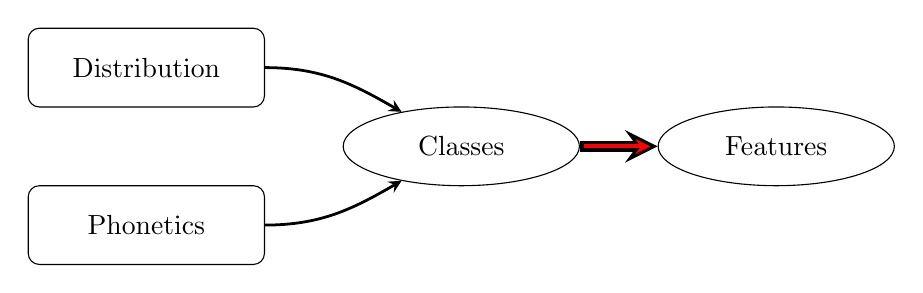
\begin{tikzpicture}[node distance=2cm, ->, >=stealth]
	\tikzstyle{input} = [rectangle, rounded corners, minimum width=3cm, minimum height=1cm,text centered, draw=black]
	\tikzstyle{output} = [ellipse, minimum width=3cm, minimum height=1cm,text centered, draw=black]
	\node (phonetics)[input] at (0, 0) {Phonetics};
	\node (distribution)[input] at (0, 2) {Distribution};
	\node (classes)[output] at (4, 1) {Classes};
	\node (features)[output] at (8, 1) {Features};
	\draw [->, out=0, in=-150, line width = 1] (phonetics) edge (classes);
	\draw [->, out=0, in=150, line width = 1] (distribution) edge (classes);
	\draw [double arrow = 4pt colored by black and red] (classes) -- (features);
	\end{tikzpicture}
	\caption{A schematic representation of the model of feature learning assumed here. This paper focuses on the red arrow between `classes' and `features'.}
	\label{fig:learning_model}
\end{figure} 

We believe that this shift is motivated. Rather than constructing models that generate the typology and subsequently concerning ourselves with the exceptions, we think that deeper insights into speech may be gained by focusing on the mechanisms by which learners identify common properties between sounds in their language, and how these mechanisms contribute to the typological patterns we see. 

Models of phonological class learning have been presented for various modalities. We are not aware of any proposals to date which have been fleshed out enough to be carefully tested, and which have proven empirically adequate. For example, \citeA{Lin2005} showed that unsupervised clustering on acoustic data was able to distinguish manner of articulation well, but not place. Conversely, unsupervised clustering on articulatory data is better able to distinguish place features, but poor at manner \cite{Mielke2012}. Such phonetically-based methods are able (in principle) to identify features corresponding to acoustic, articulatory, or perceptual properties, but these provide limited insights into the phonetically disparate classes described in the introduction, and into which classes are phonologically active in a particular language. 

Conversely, while distributional approaches \cite<e.g.,>{GoldsmithXanthos2009,Calderone2009,MayerSubmitted} have the potential (in principle) to identify both phonetically coherent and phonetically disparate classes to the extent that they are reflected in their distribution, they are blind to the phonetic properties that inform speakers' intuitions about similarities between sounds, and suffer from the presence of distributional noise. 

It seems likely to us that progress towards understanding how classes are learned will come from integrating multiple sources of information, with phonetic information providing an outline of possible classes, and distributional information shedding additional light on whether and how these classes (and possibly others) are used in a language. We see potential in methods like those described in a related paper by \citeA{MayerSubmitted}, which uses a combination of vector embedding (representing sounds numerically as points in space based on their distributional properties), Principal Component Analysis, and clustering algorithms to explicitly extract classes from a corpus. Incorporating phonetic information with distributional information may improve the performance of such models. Alternatively, a Bayesian approach, where phonetic similarity serves as an initial prior on segmental classes and considerations of their distribution inform the likelihood function, may also hold promise. A challenge for the extraction of classes from phonetic data is that classes of sounds are almost always similar only on a subset of phonetic dimensions (e.g., sonorants are articulatorily heterogeneous, but have similar acoustic properties), and the use of dimensionality reduction techniques such as Principal Component Analysis is likely to be useful in teasing apart these sources of coherence.

In any case, what must be initially identified under models that assume learned and language-specific features are \textit{classes}, with features subsequently derived from their relation. Although we see the question of how phonological classes are learned as one of great interest, the focus of this paper is on how a symbolic feature system can be derived once these classes are learned (the bold, red arrow in Fig.~\ref{fig:learning_model}). In the examples presented below, we assume that the set of input classes has been generated by mechanisms such as those just described, and focus instead on how a feature system can be derived from that set. For expositional purposes, we generally use simple, fabricated class systems, though we try to make these linguistically plausible.

Because of the relatively narrow focus of this paper, it is in many ways a stepping stone towards larger research goals. The algorithms described below make concrete predictions about questions such as where underspecification should occur, to what extent generalization occurs in feature learning, and what the feature systems of languages with phonetically disparate classes might look like. These predictions can be tested using standard phonological methods, such as AGL experiments, wug tests, corpus work, etc., as well as by revisiting the existing literature. This work, while interesting and important, is well beyond the scope of the current paper. We instead limit ourselves to carefully describing the formal properties and predictions of this approach to feature learning, while pointing out possible applications to future research. Though we hope the formal results presented here are interesting in their own right, we are equally hopefully that they may serve as useful tools in more general phonological research.

\FloatBarrier
\section{Definitions and notation}
\label{sec:definitions}
We will begin by providing a detailed notation for feature systems. This will allow us to prove several properties of these systems that are crucial for the operation of the featurization algorithms described in later sections.

\subsection{Class systems}

Let $\Sigma$ denote an alphabet of segments. We use the term \textit{class} to mean a subset of $\Sigma$. 

\vspace{0.5\baselineskip} \noindent \textbf{Definition}: A \textit{class system} $(C, \Sigma)$ consists of an alphabet $\Sigma$ and a set of classes $C$ over that alphabet. 

\vspace{0.5\baselineskip}  \noindent A simple class system, meant to evoke a manner class system, is shown in Table~\ref{table:manner_system}.

\begin{table}[htb!]
	\centering
	\begin{tabular}{|l|l|}
		\hline
		\textit{alphabet} & \{V, G, L, N, T\} \\
		\hline
		\textit{sonorants} & \{V, G, L, N\} \\
		\hline
		\textit{non-continuants} & \{N, T\} \\
		\hline
		\textit{continuants} & \{V, G, L\} \\
		\hline
		\textit{singletons} & \{V\}, \{G\}, \{L\}, \{N\}, \{T\} \\
		\hline
	\end{tabular}
	\caption{Manner hierarchy class system}
	\label{table:manner_system}
\end{table}

\subsection{Feature systems}

\textbf{Definition}: A \textit{feature system} is a tuple $(F, \Sigma, V)$ where
\begin{itemize}
    \item $\Sigma$ is a segmental alphabet, 
    \item $V$ is a set of values, and 
    \item $F$ is a \textit{featurization}: a set of features $\{f_j\}_{j=1}^M$, where each feature is a function $f: \Sigma \rightarrow V$ mapping segments to feature values.
\end{itemize}
A possible feature system for the manner system in Table~\ref{table:manner_system} is shown in Table~\ref{table:featurization}.

\begin{table}[h]
    \centering
    \begin{tabular} {|c||c|c|c|c|}
    \hline
        $\sigma$ & syl & cons & apprx & son \\ \hline
        V & + & -- & + & + \\
        G & -- & -- & + & + \\
        L & -- & + & + & + \\
        N & -- & + & -- & + \\
        T & -- & + & -- & -- \\
        \hline
    \end{tabular}
    \caption{Example of a feature system. Rows represent segments, columns represent feature functions, and cells represent feature function values for each segment.}
    \label{table:featurization}
\end{table}

\subsection{Featural descriptors}

Featural descriptors relate class and feature systems. Let $(F, \Sigma, V)$ be a feature system. We restrict $V$ to the following possibilities, whose names are intended to invoke ideas from the research literature on underspecification \cite<e.g.,>{Archangeli1988}:
\begin{itemize}
    \item \textit{privative specification}: $V = \{ +, 0 \}$
    \item \textit{full specification}: $V = \{ +, - \}$
    \item \textit{contrastive specification}: $V = \{ +, -, 0 \}$
\end{itemize}

\noindent We will use the notation $V_{spec}$ for the set $V \setminus \{0\}$, where $\setminus$ is the set difference operator. Thus $V_{spec}$ is the value set minus the zero value, or the set of non-zero values. This is because zero values are a formal mechanism to achieve underspecification, and the theoretical driver for underspecification is the idea that underspecified features are phonologically inactive (i.e., cannot define classes). Then, a \textit{featural descriptor} $\mathbf{d}$ is a set of feature/value pairs where the values cannot be $0$: i.e., $\mathbf{d} \subset V_{spec} \times F$ (where $V_{spec} \times F$ is the set of all pairs $(v,f)$ where $v \in V_{spec}$ and $f \in F$). 

For example, $\mathbf{d} =$  \featmattwo{--cons}{+son} is a featural descriptor. This is an \textit{intensional} description of a class; that is, a description of a class in terms of its properties. The \textit{extension} of a featural descriptor is the set of segments which match (at least) the feature/value pairs in the descriptor. We use angle brackets to indicate this:
$$ \big \langle \mathbf{d} \big \rangle = \{x \in \Sigma \, \mid \, \forall (\alpha_k, f_k) \in \mathbf{d} \text{,  } [ f_k(x) = \alpha_k ] \} $$
In prose, this equation says that $\big \langle \mathbf{d} \big \rangle$ is the set of all segments in $\Sigma$ such that, for every feature in $\mathbf{d}$, the value of the feature for that segment is the same as the value in $\mathbf{d}$. Note that under this definition, the extension of the empty featural descriptor is $\Sigma$, since the predicate is vacuously true for all segments when $\mathbf{d}$ is empty. 

We use the notation $V_{spec}^F$ to denote the powerset of $V_{spec} \times F$, i.e., the set of all licit featural descriptors. Lastly, we define $\langle V_{spec}^F \rangle = \{ \langle \mathbf{d} \rangle \, \mid \, \mathbf{d} \in V_{spec}^F \}$, the set of all classes described by some featural descriptor in $V_{spec}^F$. We say that the feature system $(F, \Sigma, V)$ generates the class system $\langle V_{spec}^F \rangle$.

While every featural descriptor in $V_{spec}^F$ picks out a class in $\langle V_{spec}^F \rangle$, the two are not generally in 1-1 correspondence. This is because the same class can often be described by multiple featural descriptors. For example, under the the feature system of Table~\ref{table:featurization}, the featural descriptor \featmat{--cons} picks out the same class as \featmattwo{--cons}{+son}, namely \{V, G\}. Moreover, the featural descriptors \featmattwo{+syl}{--syl} and \featmattwo{+syl}{--son} both pick out the empty set.

A feature system $(F, \Sigma, V)$ \textit{covers} a class system $(C, \Sigma)$ if $C \subseteq \langle V_{spec}^F \rangle$; in other words if the feature system provides a distinct representation for every class in $C$. 

In the next subsection, we work an example to illustrate the importance of the choice of the value set in feature systems.

\subsection{Example: Sonorants and obstruent voicing}

In this section we introduce a simple, three-segment class system to illustrate the notation, as well as the difference between the privative, full, and contrastive specification value sets.

% tables with featurization of sonorants, voiced obstruents, and voiceless obstruents
\begin{table}[h]
	\centering
	\begin{tabular}{p{5cm}p{5cm}p{5cm}}
	\begin{tabular} {|c||c|c|}
		\hline
		$\sigma$ & son & voice \\ \hline
		R & + & + \\
		D & 0 & + \\
		T & 0 & 0 \\
		\hline
	\end{tabular} &
	\begin{tabular} {|c||c|c|}
		\hline
		$\sigma$ & son & voice \\ \hline
		R & + & + \\
		D & -- & + \\
		T & -- & -- \\
		\hline
	\end{tabular} &
	\begin{tabular} {|c||c|c|}
		\hline
		$\sigma$ & son & voice \\ \hline
		R & + & 0 \\
		D & -- & + \\
		T & -- & -- \\
		\hline
	\end{tabular}
	\end{tabular}
	\caption{Sonorants and obstruents with privative (left), full (middle), and contrastive (right) specification.}
	\label{table:son_obs_features}
\end{table}

Let $\Sigma =$ \{R, D, T\}, where R is meant to evoke a sonorant, D a voiced obstruent, and T a voiceless obstruent. We begin with the featurization using the privative value set, shown on the left in Table~\ref{table:son_obs_features}. This defines three unique classes, including the alphabet. Using the simplest featural descriptors for each class, $\langle$\featmat{}$\rangle = $\{R, D, T\},  $\langle$\featmat{+son}$\rangle = $\{R\}, and $\langle$\featmat{+voice}$\rangle =$\{R, D\}. Note that this featurization provides (i) no featural descriptor that uniquely picks out the voiceless obstruent \{T\}, (ii) no way to pick out the obstruents \{T\} and \{D\} to the exclusion of \{R\}, (iii) no way to pick out the voiced obstruent \{D\} without \{R\}, and (iv) no way to pick out the empty set.

Next, consider the featurization in which the `$0$'s from the privative set are replaced with `$-$'s. This is the full specification value set. A featurization of $\Sigma$ using this set is shown in the middle in Table~\ref{table:son_obs_features}.  While the privative featurization just covers three classes, the full specification featurization covers six (not counting the empty set). Referring to `--' values provides a greater number of ways to `slice and dice' the alphabet. It follows that featurizations which assign more `$0$' values generally (though not always) require more distinct feature functions to cover the same class system. Note however that the full featurization is still restrictive, in the sense that it does not allow any arbitrary subset of segments to be identified: for example, we cannot specify \{R, T\} to the exclusion of \{D\}.

Finally, we can strike a balance in expressivity between the privative and full value sets by allowing features to take `$+$', `$-$', and `$0$' values. This is the contrastive value set. A possible contrastive featurization of $\Sigma$ is shown on the right in Table~\ref{table:son_obs_features}. Under this featurization, \featmat{voice} is now ternary, contrasting only for obstruents \cite<e.g.,>{Kiparsky1985}. This featurization picks out the same classes as the full featurization, minus the class \{R, D\}.

\subsection{Parent/child relationships in class systems}

Because the classes in a class system fall into subset/superset relationships with one another, we can represent them hierarchically. An example for the manner system in Table~\ref{table:manner_system} is shown in Fig.~\ref{fig:manner_input}. Each node in this figure is a class. Downward arrows indicate a \textit{parent/child} relationship between the connected classes. The parent/child relationship is of central importance to this work, so we formalize it carefully.

\vspace{0.5\baselineskip} \noindent \textbf{Definition}: Let $(C, \Sigma)$ be a class system. $X \in C$ is a \textit{parent} of $Y \in C$ (and $Y$ is a \textit{child} of $X$) if and only if $Y \subset X$, and there exists no $Z \in C$ such that $Y \subset Z \subset X$

\vspace{0.5\baselineskip} \noindent In other words, $X$ is a parent of $Y$ if a subset/superset relation holds, and there is no intervening class between them.

% show an example of a class system: a manner hierarchy
\begin{figure}[htb!]
	\centering
	\includegraphics[width=0.3\textwidth]{manner_poset_privative.png}
	\caption{A manner hierarchy class system.}
	\label{fig:manner_input}
\end{figure}

In Fig.~\ref{fig:manner_input}, there is a path from the alphabet through the sonorants to the continuants. This means the sonorants are a child of the alphabet, and the continuants are a child of the sonorants. This path implies the continuants are a subset of the alphabet,\footnote{Formally, the subset/superset relation is the \textit{transitive closure} of the parent/child relation, and the parent/child relation is the \textit{transitive reduction} of the subset/superset relation.} but crucially, the continuants are not a child of the alphabet because the sonorants intervene. We  define the functions $\textsc{parents}_C(Y)$ as the set of classes which are parents of a class $Y \in C$, and $\textsc{children}_C(Y)$ as the set of classes which are children of $Y \in C$.

Note that the empty set is technically a child of the singletons (since it is a subset of everything) but it does not appear in the graph. This is because the empty set is a phonologically irrelevant class: it cannot partition the alphabet into segments which pattern together and those which do not. To say that it is equivalent to the source or target of a process is equivalent to saying that the process does not happen at all.\footnote{Some confusion may arise with regard to SPE-style rules. In SPE, the null set symbol is used to indicate the source/target of epenthesis/deletion rules. Thus, in SPE the null set symbol is used to denote an \emph{empty string}. In the present work, the null set symbol is used to denote the null set.} For this reason, we generally omit the empty set throughout this paper.

One reason that we depict parent/child relationships (rather than subset/superset) is to avoid crowding the graph with arrows. But there is an additional, theoretical reason that will be crucial for the featurization algorithms we define later -- roughly speaking, in order to build a covering feature system for a set of input classes, a new feature/value pair is required only in cases where a class has exactly one parent. However, this does not hold for any class system, but only for a class system that is \textit{intersectionally closed}. The next section describes this important concept and its implications for feature systems.

\FloatBarrier
\section{Intersectional closure}
\label{sec:intersectional}

The intersectional closure of a class system $C$ is the set of classes that can be generated by intersecting an arbitrary subset of classes in $C$. We relate the intersectional closure to features by showing that if a feature system is expressive enough to generate all the classes in $C$, it necessarily generates the intersectional closure of $C$. This is a consequence of the familiar process of combining featural descriptors (also called feature bundles), where the union a set of featural descriptors defines the class that is the intersection of the classes they pick out individually. We formalize this carefully in order to prove a less obvious result: when generating a feature system from an input class system, a new feature/value pair must be added for all and only the classes that have a single parent in the intersectional closure of the input. This is because a class with more than one parent can be expressed as the union of its parents' featural descriptors.

\subsection{Definitions}

\textbf{Definition}: A collection of sets $C$ is \textit{intersectionally closed} if and only if for all $X \in C$ and $Y \in C$, $X \cap Y \in C$.

\vspace{0.5\baselineskip} \noindent The \textit{intersectional closure} of a class system $(C, \Sigma)$, written $C_\cap$, is the smallest intersectionally closed class system which contains $C$ and $\Sigma$.

\vspace{0.5\baselineskip} \noindent \textbf{Definition}: $C_\cap = \{ \, \bigcap P \, \mid \, P \subseteq C\} \cup \{\Sigma\}$

\vspace{0.5\baselineskip} \noindent where $P$ ranges over every subset of the classes in $C$ and $\bigcap P$ indicates the intersection of all classes in $P$. In other words, the intersectional closure contains every class which can be generated by finite intersections of classes from $C$ (and $\Sigma$), and no other classes besides these.

To illustrate this concept, we introduce the vowel inventory in Table~\ref{table:vowel_inventory} and a possible class system over this inventory in Table~\ref{table:vowels1}. This class system will serve as a running example throughout the rest of the paper. It is intended to strike a balance between linguistic plausibility and simplicity for expositional purposes.

\begin{table}[h]
    \centering
    \begin{tabular} {|c|c|c|c|}
    \hline
                 &            front                   & central           & back         \\ \hline
         high & \textipa{i} \textipa{y}      &                  & \textipa{u} \\
         mid  & \textipa{e} \textipa{\o} &                  & \textipa{o} \\
         low  &                                       & \textipa{a} &                  \\ \hline
    \end{tabular}
    \caption{Vowel inventory}
    \label{table:vowel_inventory}
\end{table}

\begin{table}[h]
	\centering
	\begin{tabular} {|l|l|}
		\hline
		\textit{alphabet} & \{\textipa{a}, \textipa{i}, \textipa{u}, \textipa{e},  \textipa{o}, \textipa{y}, \textipa{\o}\} \\
		\hline
		\textit{non-low} & \{\textipa{i}, \textipa{u}, \textipa{e},  \textipa{o}, \textipa{y}, \textipa{\o}\} \\
		\hline
		\textit{high} & \{\textipa{i}, \textipa{u}, \textipa{y}\} \\
		\hline
		\textit{front} & \{\textipa{i}, \textipa{e}, \textipa{y}, \textipa{\o}\} \\
		\hline
		\textit{round} & \{\textipa{u}, \textipa{o}, \textipa{y}, \textipa{\o}\} \\
		\hline
		\textit{singletons} & \{\textipa{a}\}, \{\textipa{i}\}, \{\textipa{u}\}, \{\textipa{e}\}, \{\textipa{o}\}, \{\textipa{y}\}, \{\textipa{\o}\} \\
		\hline
	\end{tabular}
	\caption{Vowel classes}
	\label{table:vowels1}
\end{table}

Let $(C, \Sigma)$ consist of the classes in Table~\ref{table:vowels1}. $(C, \Sigma)$ and $C_\cap$ are depicted in Fig.~\ref{fig:vowel_inventory}. The difference between the two is highlighted by using red ovals for the `extra' classes.

% FIGURE 2
\begin{figure}[h]
  \centering
  \subfloat{{\includegraphics[width=0.45\textwidth]{vowel_inventory_base.png}}}
  \qquad
  \subfloat{{\includegraphics[width=0.45\textwidth]{vowel_inventory_closure.png}}}
  \caption{The original vowel system (left) and its intersectional closure (right). Classes added in the closure are indicated with red ovals. Dotted lines in the intersectional closure indicate classes with more than one parent.}
  \label{fig:vowel_inventory}
\end{figure}

% Old figure setup
%% FIGURE 2
%\begin{figure}[h]
%	\centering
%	\includegraphics[width=0.8\textwidth]{vowel_inventory_base.png}
%	\caption{A vowel inventory.}
%	\label{fig:vowel_inventory}
%\end{figure}
%
%% FIGURE 3
%\begin{figure}[h]
%	\centering
%	\includegraphics[width=0.7\textwidth]{vowel_inventory_closure.png}
%	\caption{Intersectional closure of the vowel inventory. Classes added in the closure are indicated with red ovals.}
%	\label{fig:vowel_inventory_closure}
%\end{figure}

The key difference is that the intersectional closure contains several two-segment classes which are the intersection of larger classes. For example, the \textit{high, front} class \{\textipa{i}, \textipa{y}\} is the intersection of the \textit{high} class and the \textit{front} class:
$$ \text{\{\textipa{i}, \textipa{y}\}} = \text{\{\textipa{i}, \textipa{y}, \textipa{u}\}} \cap \text{\{\textipa{i}, \textipa{y}, \textipa{e}, \textipa{\o}\}} $$
In the next section, we prove that if a feature system is expressive enough to cover $C$, it also covers $C_\cap$.

\subsection{Feature systems generate an intersectional closure}

There is a dual relationship between featural descriptors and the classes they describe: intersection of classes corresponds to union of featural descriptors. We formalize this property with a lemma and then provide a concrete example. An important consequence of the following lemma is that it entails that if a featurization covers $C$, it must also cover the intersectional closure $C_\cap$. We prove this in the theorem that follows.

\begin{clump}
\vspace{\baselineskip} \noindent \textbf{Featural Intersection Lemma}

\indent Let $(F, \Sigma, V)$ be a feature system. If $\mathbf{d}_i, \mathbf{d}_j \in V_{spec}^F$, then $\langle \mathbf{d}_i \cup \mathbf{d}_j \rangle =  \langle \mathbf{d}_i \rangle \cap \langle \mathbf{d}_j \rangle$.
\end{clump}

\noindent \textit{Proof}:

The proof proceeds by showing that $ \langle \mathbf{d}_i \rangle \cap \langle \mathbf{d}_j \rangle \subseteq \langle \mathbf{d}_i \cup \mathbf{d}_j \rangle$ and $\langle \mathbf{d}_i \cup \mathbf{d}_j \rangle \subseteq \langle \mathbf{d}_i \rangle \cap \langle \mathbf{d}_j \rangle$.
Let $C_i = \langle \mathbf{d}_i \rangle$ and $C_j = \langle \mathbf{d}_j \rangle$.
First, suppose $x \in C_i \cap C_j$. Then $x \in C_i$. By definition, $x$ has the features in $\mathbf{d}_i$.
Similarly, $x \in C_j$, and therefore must have the features in $\mathbf{d}_j$.
Thus, $x$ has the features in $\mathbf{d}_i \cup \mathbf{d}_j$. This shows that $C_i \cap C_j \subseteq \langle \mathbf{d}_i \cup \mathbf{d}_j \rangle$.
Now, suppose $x \in \langle \mathbf{d}_i \cup \mathbf{d}_j \rangle$. Then $x$ has all the features of $\mathbf{d}_i$, and so $x \in C_i$.
Similarly, $x$ has all the features of $\mathbf{d}_j$, so $x \in C_j$. Therefore $x \in C_i \cap C_j$. This shows that $\langle \mathbf{d}_i \cup \mathbf{d}_j \rangle \subseteq C_i \cap C_j$.
Since both $C_i \cap C_j$ and $\langle \mathbf{d}_i \cup \mathbf{d}_j \rangle$ are subsets of each other, they are equal.
$\square$

\vspace{0.5\baselineskip} We illustrate this lemma with reference to the vowel inventory system introduced above. For concreteness, let us adopt the featurization in Table~\ref{table:vowel_inventory_underspec}.

% table with featurization of sonorants, voiced obstruents, and voiceless obstruents
\begin{table}[h]
    \centering
    \begin{tabular} {|c||c|c|c|c|}
    \hline
        $\sigma$      & low & front & round & high \\ \hline
        \textipa{a}    & +          & 0      & 0         & 0       \\
        \textipa{i}      & --          & +      & 0        & +      \\        \textipa{u}    & --          & --      & +         & +      \\
        \textipa{e}    & --          & +      & 0         & --      \\
        \textipa{o}    & --          & --      & +         & --      \\ 
        \textipa{\o} & --          & +      & +         & --      \\
        \textipa{y}    & --          & +      & +         & +       \\ \hline
    \end{tabular}
    \caption{A featurization of the vowel inventory. The low vowel is unspecified for front/round/high features; the round feature is privative.}
    \label{table:vowel_inventory_underspec}
\end{table}

\noindent Let $\mathbf{d}_1 =$ \featmat{+front} and $\mathbf{d}_2 =$ \featmat{+round}. Then we have: \begin{itemize}
    \item $\langle \mathbf{d}_1 \rangle = \langle$\featmat{+front}$\rangle =$ \{\textipa{i}, \textipa{e}, \textipa{y}, \textipa{\o}\}
    \item $\langle \mathbf{d}_2 \rangle = \langle$\featmat{+round}$\rangle =$ \{\textipa{u}, \textipa{o}, \textipa{y}, \textipa{\o}\}
    \end{itemize}
\noindent For these values, the Featural Intersection Lemma cashes out as follows: `the set of vowels that are both front and round' is the intersection of `the set of vowels that are front' and `the set of vowels that are round':
 
\begin{itemize}
    \item $\langle \mathbf{d}_1 \rangle \cap \langle \mathbf{d}_2 \rangle =  \langle$\featmat{+front}$\rangle \cap \langle$\featmat{+round}$\rangle =$\{\textipa{i}, \textipa{e}, \textipa{y}, \textipa{\o}\} $\cap$ \{\textipa{u}, \textipa{o}, \textipa{y}, \textipa{\o}\} = \{\textipa{y}, \textipa{\o}\}
    \item $\langle \mathbf{d}_1 \cup \mathbf{d}_2 \rangle = \langle$\featmattwo{+front}{+round}$\rangle =$ \{\textipa{y}, \textipa{\o}\}
\end{itemize}

\noindent The Featural Intersection Lemma proves that this kind of relationship holds for any pair of featural descriptors and the classes they describe.

An important consequence of this lemma is that it can be applied inductively, to relate the union of multiple featural descriptors with the intersection of multiple classes. Because the intersectional closure is defined as the intersection of arbitrarily many classes in an input $C$, the Featural Intersection Lemma entails that if a featurization covers $C$, it must cover the intersectional closure.

\begin{clump}
\vspace{\baselineskip} \noindent \textbf{Intersectional Closure Covering Theorem}

\noindent Let $(C, \Sigma)$ be a class system and $(F, \Sigma, V)$ a feature system. If $C \subseteq \langle V_{spec}^F \rangle$, then $C_\cap \subseteq \langle V_{spec}^F \rangle $.
\end{clump}
\noindent \textit{Proof}:

Let $Y$ be an arbitrary class in $C_\cap$. By definition of $C_\cap$, there exist $\{X_i \in C\}_{i \in I}$ (for some index set $I$, hereafter omitted) such that $Y = \bigcap_i \, X_i$. The hypothesis that $C \subseteq \langle V_{spec}^F \rangle $ implies that for every such $X_i$, there is a featural descriptor $\mathbf{d}_i$ such that $\langle \mathbf{d}_i \rangle = X_i$. Thus, $Y = \bigcap_i X_i = X_1 \cap X_2 \cap \ldots \cap X_n$ can also be written $Y = \bigcap_i \, \langle \mathbf{d}_i \rangle = \langle \mathbf{d}_1 \rangle \cap \langle \mathbf{d}_2 \rangle \cap \ldots \cap \langle \mathbf{d}_n \rangle$. It follows by induction using Featural Intersection Lemma that $Y = \langle \bigcup_i \mathbf{d}_i \rangle$:

$Y = \langle \mathbf{d}_1 \rangle \cap  \langle \mathbf{d}_2 \rangle \cap \ldots \cap  \langle \mathbf{d}_n \rangle$

\quad $ = \langle \mathbf{d}_1 \cup \mathbf{d}_2 \rangle \cap \mathbf{d}_3 \cap \ldots \cap \langle \mathbf{d}_n \rangle$

\quad $ = \langle \mathbf{d}_1 \cup \mathbf{d}_2 \cup \mathbf{d}_3 \rangle \cap \ldots \cap \langle \mathbf{d}_n \rangle$

\quad $\ldots$

\quad $= \langle \mathbf{d}_1 \cup \mathbf{d}_2 \cup \ldots \cup \mathbf{d}_n \rangle$

\quad $= \langle \bigcup_i  \mathbf{d}_i \rangle$

\noindent The preceding chain of logic demonstrates the following fact: if a class can be expressed as the intersection of classes in $C$, then its features are the union of the features in each of those classes. The intersectional closure is defined as all possible intersections of classes in $C$. Thus, because $(\bigcup_i \mathbf{d}) \in V_{spec}^f$, if $(F, \Sigma, V)$ covers $C$, it covers the intersectional closure. $\square$

\vspace{0.5\baselineskip} A dynamic programming algorithm for efficiently calculating the intersectional closure of a set of classes is presented in Appendix~\ref{app:closure}.

\subsection{Parenthood in the intersectional closure}
\label{sec:intersection_proof}

The intersectional closure not only characterizes the expressiveness of a featurization, but is also instrumental in deriving featurizations from a class system. When generating a feature system from a set of classes, \textit{a new feature/value pair is required for all and only the classes which have a single parent in the intersectional closure}. The reason for this is that if a class has two parents, it must be their intersection.

\begin{clump}
\vspace{\baselineskip} \noindent \textbf{Multiple Parenthood Theorem}

\noindent Let $(C, \Sigma)$ be a class system and $Y \in C_\cap$. If $X_1, X_2 \in \textsc{parents}_C(Y)$, then $Y = X_1 \cap X_2$.
\end{clump}

\noindent \textit{Proof}:

First, observe that $Y \subseteq X_1 \cap X_2$. This follows trivially from the definition of parenthood: $X_1$ is a parent of $Y$ implies $Y \subset X_1$; $X_2$ is a parent of $Y$ implies $Y \subset X_2$; and so every element in $Y$ is in both $X_1$ and $X_2$.

Now suppose that $X_1 \cap X_2 \neq Y$. The preceding logic showed that either the two are equal, or $Y$ is a proper subset of $X_1 \cap X_2$. But the latter case creates a contradiction. By definition, $X_1 \cap X_2$ must be in the intersectional closure. It must also be the case that $X_1 \cap X_2 \subset X_1$. If $X_1 \cap X_2 = X_1$ then $X_2$ is either identical to or a supserset of $X_1$, contradicting the assumption that $X_1$ and $X_2$ are parents of $Y$, and $X_1 \cap X_2 \supset X_1$ is ruled out by the fundamental properties of sets. Thus $X_1 \cap X_2$ intervenes between $Y$ and $X_1$, contradicting the hypothesis that $Y$ is a daughter of $X_1$. Thus, $Y = X_1 \cap X_2$. $\square$

\vspace{0.5\baselineskip} Note that the Multiple Parenthood Theorem does not logically exclude the possibility that a class may have more than two parents. Rather, it guarantees that in such cases, the intersection is the same so long as two or more parents are considered. A case of this arose already in Fig.~\ref{fig:vowel_inventory}, in the intersectional closure of the vowel inventory. There, the three features \textit{front}, \textit{high}, and \textit{round} give rise to three distinct 2-feature classes (featural descriptors: \featmattwo{+front}{+high}, \featmattwo{+high}{+round}, \featmattwo{+front}{+round}). The intersection of any pair of these is \{\textipa{y}\} (the high, front, round vowel). Thus, the set  \{\textipa{y}\} has three parents, but which segments it contains is uniquely determined by any two of them.

\subsection{Interim summary}

In Section~\ref{sec:definitions}, we defined a formal notation for class systems, feature systems, and featural descriptors, and explored the expressiveness of different value sets in feature systems. In Section~\ref{sec:intersectional}, we proved that any feature system that is expressive enough to cover a class system necessarily covers the intersectional closure of that class system. We then showed that if a class has more than one parent in the intersectional closure of a class system, it is the intersection of any two of those parents. This latter point will be the key element of the featurization algorithms described in the rest of the paper.

With the necessary components in place, we now turn to the main question addressed in this paper: given a set of phonological classes, how can we generate a covering feature system? We detail four algorithms that accomplish this, differing in their assumptions about which value sets are used and how these values are assigned.

\FloatBarrier
\section{Generating a feature system from a set of input classes}
\label{sec:algorithm_intro}

In this section, we will detail the operation of four algorithms that generate a feature system from a set of input classes. The basic principle these algorithms share is that we must introduce a new feature/value pair for each class in the intersectional closure that has a single parent. This is because classes with more than one parent may be specified by the union of the features of any two of their parents, and so do not need a new feature to distinguish them from their parents. The four algorithms differ in which value sets they use and how they assign these values.

We will use the simple class system shown in Fig.~\ref{fig:toy_system} to illustrate the properties of each algorithm. This system is intersectionally closed. Note that this system does not include all of the singleton classes. This is equivalent to removing the stipulation that the resulting feature system must be able to pick out each segment individually. Although this is doubtless a desirable property in real phonological systems, we relax it here for expositional purposes. The next section will provide a substantive discussion of the theoretical implications of each featurization type using a more realistic input.

\begin{figure}[htb!]
	\centering
	\includegraphics[width=0.2\textwidth]{toy_system.png}
	\caption{A toy class system.}
	\label{fig:toy_system}
\end{figure}

The notation used to define the algorithms may be unfamiliar to some readers. Table~\ref{table:algorithm_definitions} provides definitions for some of the less obvious terms. The rest of the notation should be familiar from basic set theory.

\begin{table}
	\centering
	\begin{tabular}{|l|p{9cm}|}
		\hline
		\textbf{Require} & Expresses constraints on the input \\
		\hline
		\textbf{Ensure} & Expresses constraints on the output \\
		\hline
		\begin{tabular}[t]{@{}l}
		$Q$ \\
		\textsc{dequeue} \\
		\textsc{enqueue}
		\end{tabular} & $Q$ is a queue, which is a set of ordered values. Queues are ``first in, first out'', which means values are removed from the queue using \textsc{dequeue} in the same order they were added to the queue using \textsc{enqueue}. Statements like $Q \leftarrow C_\cap$ indicate that the sets in $C_\cap$ are added to $Q$ in an arbitrary order.\\
		\hline
		\textsc{IntersectionalClosure} & Returns the intersectional closure of the input class system. $Q'$ indicates the starting state of the queue (see Appendix~\ref{app:closure}). \\
		\hline
	\end{tabular}
	\caption{Definitions for some terms used in algorithms.}
	\label{table:algorithm_definitions}
\end{table}

\subsection{Privative specification}

The first algorithm yields a \textit{privative} featurization of a set of classes: that is, one where the set of legal feature values $V = \{+, 0\}$. It does so by assigning a different feature/value pair, \featmat{$+f$}, to the segments in each class with a single parent.

\noindent \begin{algorithmic}
	\singlespacing
    \REQUIRE $C_\cap$ is the intersectional closure of a class system $(C, \Sigma)$
    \ENSURE $F$ is a featurization over $V = \{ +, 0 \}$ which covers $C$
    \STATE
    \STATE $Q \leftarrow C_\cap$
    \STATE $F \leftarrow \varnothing$
    \STATE
    \WHILE{$Q \neq \varnothing$}
        \STATE $X \leftarrow \textsc{dequeue}(Q)$
        \IF{$|\textsc{parents}_C(X)| = 1$}
            \STATE define $f_X : \Sigma \rightarrow V$ by $f_X(\sigma) = \begin{cases}
                + & \mbox{if } \sigma \in X \\
                0 & \mbox{otherwise}
                \end{cases} $
            \STATE $F \leftarrow F \cup \{f_X\}$
        \ENDIF
    \ENDWHILE
\end{algorithmic}
\doublespacing

\noindent \textit{Proof of soundness for the privative specification algorithm}

A featurization algorithm is \textit{sound} if for every class system $(C, \Sigma)$, it returns a feature system which covers $C$. To see that the privative specification algorithm is sound, note that every class in $C_\cap$ enters the queue $Q$. For an arbitrary class $X$ in the queue, there are three cases. If $X$ has 0 parents, then it is $\Sigma$, and is covered by the empty featural descriptor. If $X$ has exactly 1 parent, then the segments in $X$ will have the features of that parent (which uniquely pick out the parent class), plus a new feature $f$ which distinguishes the segments in $X$ from $X$'s parent. If $X$ has more than 1 parent, then Multiple Parenthood Theorem shows, via the Featural Intersection Lemma, that the union of features of $X$'s parents uniquely pick out all and only the segments in $X$. Thus, each class which exits the queue has a set of features assigned to its segments which pick out that class uniquely. This completes the proof. $\square$

\begin{figure}[htb!]
	\centering
	\begin{minipage}{0.45\textwidth}
		\centering
		\includegraphics[width=0.45\textwidth]{toy_system_privative.png}
		\caption{Yield of the privative specification algorithm.}\label{fig:toy_system_privative}
	\end{minipage}
	\begin{minipage}{0.45\textwidth}
		\centering
		\captionsetup{type=table} %% tell latex to change to table
		\begin{tabular} {|c||c|c|c|}
			\hline
			$\sigma$ & F1 & F2 & F3 \\ \hline
			a & + & 0 & 0 \\
			b & 0 & + & + \\
			c & 0 & + & 0  \\
			\hline
		\end{tabular}
		\caption{Featural specification of the toy system with privative specification.}\label{table:toy_system_privative}
	\end{minipage}
\end{figure}

%\begin{figure}[htb!]
%	\centering
%	\includegraphics[width=0.2\textwidth]{toy_system_privative.png}
%	\caption{Yield of the privative specification algorithm.}
%	\label{fig:toy_system_privative}
%\end{figure}

%\begin{table}[h]
%	\centering
%	\begin{tabular} {|c||c|c|c|}
%		\hline
%		$\sigma$ & F1 & F2 & F3 \\ \hline
%		a & + & 0 & 0 \\
%		b & 0 & + & + \\
%		c & 0 & + & 0  \\
%		\hline
%	\end{tabular}
%	\caption{Featural specification of the toy system with privative specification.}
%	\label{table:toy_system_privative}
%\end{table}
The output of this algorithm on the simple class system in Fig.~\ref{fig:toy_system} is shown in Fig.~\ref{fig:toy_system_privative}. The visual style is similar, but this figure contains additional annotations for the feautures themselves. The boxes which represent the classes contain the segments in the class, followed by the list of features that are shared by all segments in the class. Recall that if a class has a feature, all descendants of the class share that feature. The introduction of a feature is thus indicated explicitly by labeling and coloring the edge which points to the first/highest class whose segments share the feature. This could give the misleading impression that features are assigned to classes, so it is worth reiterating that features are maps from \textit{segments} to values. The complete featurization of each individual segment is given in Table~\ref{table:toy_system_privative}. Each class with a single parent has resulted in a new feature/value pair being generated, resulting in a total of three features.

\FloatBarrier
\subsection{Complementary specification}
\label{sec:contrastiveunder}

It is common for theoretical reasons to assign corresponding $\pm$ feature values to pairs of classes, such as \featmat{+back} and \featmat{$-$back} vowels. Such binary features are often relevant for only certain segments (e.g., we may want to only specify voicing for obstruents, backness for dorsal sounds, and so on). In all such cases, the contrastive feature values denote \textit{complementary} classes -- but complements with respect to \textit{what}?  

The central insight developed in this paper is that a new feature needs to be assigned just in case a class has a single parent in the intersectional closure. This suggests that a relevant domain for complementation is with respect to the parent. This is the distinction between privative specification and complementary specification: a `$-$' value is assigned when the complement of the class being processed with respect to its parent is in the input.
\noindent \begin{algorithmic}
	\singlespacing
    \REQUIRE $C_\cap$ is the intersectional closure of input class system $(C, \Sigma)$
    \ENSURE $F$ is a featurization over $V = \{ +, -, 0 \}$ which covers $C$
    \STATE
    \STATE $Q \leftarrow C_\cap$
    \STATE $F \leftarrow \varnothing$
    \STATE
    \WHILE{$Q \neq \varnothing$}
        \STATE $X \leftarrow \textsc{dequeue}(Q)$
        \IF{$| \textsc{parents}_C(X) | = 1$}
            \STATE $P_X \leftarrow \textsc{dequeue}(\textsc{parents}_C(X))$
            \STATE
            \STATE $\overline{X} \leftarrow \begin{cases}
                P_X \setminus X & \text{if } (P_X \setminus X) \in C \\
                \varnothing     & \text{otherwise}
                \end{cases}$
            \STATE
            \STATE define $f_X : \Sigma \rightarrow V$ by $f_X (\sigma) = \begin{cases}
                    + & \text{if } \sigma \in X \\
                    - & \text{if } \sigma \in \overline{X} \\
                    0 & \text{otherwise}
                    \end{cases}$
            \STATE $F \leftarrow F \cup \{f_X\}$
            \STATE $Q \leftarrow \{x \in Q \vert x \neq \overline{X} \}$
        \ENDIF
    \ENDWHILE
\end{algorithmic}
\doublespacing

\noindent The soundness of this algorithm follows from the soundness of the privative specification algorithm. This is because the complementary specification algorithm yields a feature system which generates the same class system as privative specification does. The difference between the two is that if the input contains complement sets, then complementary specification will use a single feature with `$+$' and `$-$' values, where privative specification will have two features with just `$+$' values.

\begin{figure}[htb!]
	\centering
	\begin{minipage}{0.45\textwidth}
		\centering
		\includegraphics[width=0.45\textwidth]{toy_system_complementary.png}
		\caption{Yield of the complementary specification algorithm.}
		\label{fig:toy_system_complementary}
	\end{minipage}
	\begin{minipage}{0.45\textwidth}
		\centering
		\captionsetup{type=table} %% tell latex to change to table
	\begin{tabular} {|c||c|c|}
	\hline
	$\sigma$ & F1 & F2 \\ \hline
	a & + & 0 \\
	b & -- & + \\
	c & -- & 0 \\
	\hline
\end{tabular}
\caption{Featural specification of the toy system with complementary specification.}
\label{table:toy_system_complementary}
	\end{minipage}
\end{figure}

%\begin{figure}[htb!]
%	\centering
%	\includegraphics[width=0.2\textwidth]{toy_system_complementary.png}
%	\caption{Yield of the complementary specification algorithm.}
%	\label{fig:toy_system_complementary}
%\end{figure}
%
%\begin{table}[h]
%	\centering
%	\begin{tabular} {|c||c|c|}
%		\hline
%		$\sigma$ & F1 & F2 \\ \hline
%		a & + & 0 \\
%		b & -- & + \\
%		c & -- & 0 \\
%		\hline
%	\end{tabular}
%	\caption{Featural specification of the toy system with complementary specification.}
%	\label{table:toy_system_complementary}
%\end{table}

The output of this algorithm on the simple class system in Fig.~\ref{fig:toy_system} is shown in Fig.~\ref{fig:toy_system_complementary}, and the complete featurization is shown in Table~\ref{table:toy_system_complementary}. Note that each class with a single parent has still been assigned a new feature/value pair. However, because the `$-$' value is available, and two classes fall into a complementary relationship with respect to their parent, we require only two features to generate the same class system.

The term \textit{complementary specification} is meant to capture the fact that specification for a particular feature occurs just for segments that are in the class that motivates the addition of the feature, or in its complement with respect to the parent if this class is in the input. In the next section, we consider a variant of the algorithm which guarantees members of such complement classes will receive `$-$' values, even if they were not present in the input. We call this variant \textit{inferential complementary specification}.

\FloatBarrier
\subsection{Inferential complementary specification}
\label{sec:contrastive}

Inferential complementary (IC) specification, like complementary specification, generates a ternary feature system. The key difference is that IC specification adds complements with respect to the parent to the set of classes. Every complement gets a `$-$' feature, \textit{including those which were not in the input}. In other words, the learner performs a limited generalization from the input classes to infer the existence of certain classes that were not in the input.

IC specification thus requires modifying the intersectional closure of the input. One way to handle this is to update the intersectional closure as features are assigned. However, it is also possible to precompute the result, because the classes that must be added can be defined in terms of subset/superset relations, which do not depend on features. We do this as it is conceptually simpler.

We denote the function that adds complement classes with \textsc{AddComplements}. When adding complement classes, the ordering in which classes are processed is crucially important. Breadth-first traversal -- processing all the siblings of a class before its children -- is done to avoid configurations that duplicate a feature. In addition, the order in which siblings are processed during breadth-first traversal has important consequences for the generated class and feature systems. We adopt a procedure whereby the complements of all siblings are added \textit{simultaneously} to the class set if they are not already present. This has the potential to result in more features than would be generated if the complements were added one-by-one as each class is processed, but it avoids imposing class hierarchies that are not motivated by the input class set. A further motivation for this scheme is that if classes are not processed simultaneously, some order must be chosen, and there is no obvious motivation for choosing one over another. A detailed description of \textsc{AddComplements} and additional discussion of the points above can be found in Appendix \ref{app:complements}.
\noindent \begin{algorithmic}
	\singlespacing
    \REQUIRE $C_\cap$ is the intersectional closure of input class system $(C, \Sigma)$
    \ENSURE $F$ is a featurization over $V = \{ +, -, 0 \}$ which covers $C$
    \STATE
    \STATE $Q \leftarrow \textsc{AddComplements}(C_\cap)$
    \STATE $F \leftarrow \varnothing$
    \STATE
    \WHILE{$Q \neq \varnothing$}
        \STATE $X \leftarrow \textsc{dequeue}(Q)$
        \IF{$| \textsc{parents}_C(X) | = 1$}
            \STATE $P_X \leftarrow \textsc{dequeue}(\textsc{parents}_C(X))$
            \STATE $\overline{X} \leftarrow P_X \setminus X$
            \STATE define $f_X : \Sigma \rightarrow V$ by $f_X (\sigma) = \begin{cases}
                    + & \text{if } \sigma \in X \\
                    - & \text{if } \sigma \in \overline{X} \\
                    0 & \text{otherwise}
                    \end{cases}$
            \STATE $F \leftarrow F \cup \{f_X\}$
            \STATE $Q \leftarrow \{x \in Q \vert x \neq \overline{X} \}$
        \ENDIF
    \ENDWHILE
\end{algorithmic}
\doublespacing

\noindent This algorithm is sound because it considers all the classes that the privative specification algorithm does, plus others. Thus, it necessarily covers $C$.

The output of this algorithm on the simple class system in Fig.~\ref{fig:toy_system} is shown in Fig.~\ref{fig:toy_system_ic}, and the complete featurization is shown in Table~\ref{table:toy_system_ic}. 

\begin{figure}[htb!]
	\centering
	\includegraphics[width=0.2\textwidth]{toy_system_ic.png}
	\caption{Yield of the IC specification algorithm. Classes added by the algorithm are indicated with dashed boxes.}
	\label{fig:toy_system_ic}
\end{figure}

\begin{table}[h]
	\centering
	\begin{tabular} {|c||c|c|}
		\hline
		$\sigma$ & F1 & F2 \\ \hline
		a & + & 0 \\
		b & - & + \\
		c & - & - \\
		\hline
	\end{tabular}
	\caption{Featural specification of the toy system with IC specification.}
	\label{table:toy_system_ic}
\end{table}

Note that, as with complementary specification, only two features are needed to cover the input. However, the learner has inferred the existence of a class \{c\}, because its complement \{b\} with respect to its parent \{b,c\} was present in the input. As a result, c is no longer unspecified for F2.

The feature system yielded by IC specification is more expressive than the ones yielded by privative or complementary specification, but it is not maximally expressive, since there are still `$0$' values. When a new feature is added, non-zero values are assigned only to classes that are descendants of the parent of the class that generates the feature. If we want to eliminate all `$0$' values, we can do complementation with respect to $\Sigma$ rather than the parent. That is the final variant -- full specification.

\FloatBarrier
\subsection{Full specification}
\label{sec:full}

Full specification differs from IC specification in that complementation is calculated with respect to the whole alphabet, rather than the parent class. Therefore, it is algorithmically almost the same as IC specification. As with IC specification, the complement classes are precomputed and added to the intersectional closure in breadth-first search order, and siblings are processed simultaneously. We denote this process as \textsc{AddComplementsFull}: see Appendix \ref{app:complements} for a detailed discussion.
\noindent \begin{algorithmic}
	\singlespacing
    \REQUIRE $C_\cap$ is the intersectional closure of input class system $(C, \Sigma)$
    \ENSURE $F$ is a featurization over $V = \{ +, - \}$ which covers $C$
    \STATE
    \STATE $Q \leftarrow \textsc{AddComplementsFull}(C_\cap)$
    \STATE $F \leftarrow \varnothing$
    \STATE
    \WHILE{$Q \neq \varnothing$}
        \STATE $X \leftarrow \textsc{dequeue}(Q)$
        \IF{$| \textsc{parents}_C(X) | = 1$}
	        \STATE $\overline{X} \leftarrow \Sigma \setminus X$
            \STATE define $f_X : \Sigma \rightarrow V$ by $f_X (\sigma) = \begin{cases}
                    + & \text{if } \sigma \in X \\
                    - & \text{otherwise}
                    \end{cases}$
            \STATE $F \leftarrow F \cup \{f_X\}$
            \STATE $Q \leftarrow \{x \in Q \vert x \neq \overline{X} \}$
        \ENDIF
    \ENDWHILE
\end{algorithmic}
\doublespacing

\noindent The full specification algorithm is sound for the same reason that the IC specification algorithm is -- it considers a superset of classes that the privative specification algorithm does, and thus it covers the input.

The output of this algorithm on the simple class system in Fig.~\ref{fig:toy_system} is shown on the left side of Fig.~\ref{fig:toy_system_full_features}, and the complete featurization is shown in Table~\ref{table:toy_system_full}. 

\begin{figure}[htb!]
	\centering
	\subfloat{{\includegraphics[width=0.3\textwidth]{toy_system_full_features_FEATURAL.png}}}
	\qquad
	\subfloat{{\includegraphics[width=0.225\textwidth]{toy_system_full_features_TOPOLOGICAL.png}}}
	\caption{Featural (left) and topological (right) plots of the output of the full specification algorithm. Classes added by the algorithm are in dashed boxes. Classes added due to the addition of these classes to the intersectional closure are not highlighted.}
	\label{fig:toy_system_full_features}
\end{figure}

%\begin{figure}[htb!]
%	\centering
%	\includegraphics[width=0.3\textwidth]{toy_system_full_features_FEATURAL.png}
%	\caption{Featural (left) and topological (right) plots of the output of the full specification algorithm. Classes added by the algorithm are indicated with dashed boxes. Classes added due to the addition of these classes to the intersectional closure are not highlighted.}
%	\label{fig:toy_system_full_features}
%\end{figure}
%
%\begin{figure}[htb!]
%	\centering
%	\includegraphics[width=0.2\textwidth]{toy_system_full_features_TOPOLOGICAL.png}
%	\caption{Topological plot of the output of the full specification algorithm.}
%	\label{fig:toy_system_full_topological}
%\end{figure}

\begin{table}[h]
	\centering
	\begin{tabular} {|c||c|c|}
		\hline
		$\sigma$ & F1 & F2 \\ \hline
		a & + & - \\
		b & - & + \\
		c & - & - \\
		\hline
	\end{tabular}
	\caption{Featural specification of the toy system with full specification.}
	\label{table:toy_system_full}
\end{table}

The resulting feature system from the full specification algorithm contains no `0' values, and so all segments are fully specified for all features. The \{a,c\} class has been added because it is the complement of \{b\} with respect to the alphabet, and the class \{c\} has been generated by intersectional closure of this new class system.

There is an important difference between this plot and previous ones. We may consider two types of plots when plotting featural relations: a \emph{topological} plot, which plots relationships between classes using the familiar notions of the parent/child relationship, and a \emph{featural} plot, where classes corresponding to \featmat{$+f$} and \featmat{$-f$} feature/value pairs are plotted as siblings. In all cases considered so far, these two plotting strategies have resulted in identical outcomes. With the full specification algorithm on the toy class system, this is no longer the case. This mismatch is the result of \featmat{$-f$} values being assigned to classes that have multiple parents and/or are not siblings of the class motivating the new feature.

The plot on the left of Fig.~\ref{fig:toy_system_full_features} is the featural plot. The topological plot is shown to the right. The most salient difference is that the \featmat{--F1} and \featmat{--F2} classes are represented as siblings of the \featmat{+F1} and \featmat{+F2} classes in the featural plot, corresponding to the structure of the feature system. The topological plot, however, shows that these classes are not in fact siblings.

We use featural plots through the rest of the paper because they are more representative of the abstract structure and relationships assigned by the feature system, which subsume the topological system to some degree. Topological plots can be found in Appendix~\ref{app:topological}. Comparing these types of plots provides some insight into how topological and featural relationships in a class system may diverge.

\subsection{Summary of the algorithms}

This section described four algorithms that take a set of input classes and return a feature system that covers that class system. All four algorithms generate a new feature/value pair for any class that has a single parent in the intersectional closure of the input class system. The privative specification algorithm generates a system using only privative values. The complementary specification algorithm generates a ternary-valued feature system by assigning $\pm$ feature values to classes in the input that are complements with respect to their single parent. The inferential complementary specification algorithm behaves similarly, but it assigns `$-$' values to complement classes with respect to a parent in every case, adding them to the input if they are not present. Finally, the full specification algorithm assigns `$-$' values to complement classes with respect to the alphabet, resulting in no `0' values being assigned.

We now illustrate the performance of these algorithms on a more plausible input class system, and discuss some of the theoretical implications of each method.

\FloatBarrier
\section{Theoretical implications of different featurizations}
\label{sec:theoretical_implications}

The examples in this section will use the vowel class inventory shown in Fig.~\ref{fig:vowel_inventory} as input. For readability we generally use familiar feature names when the feature picks out more than one segment, and the segment's name (e.g., \featmat{+i}) when the feature only picks out a single segment. These single segment features are a consequence of the singleton sets being included in the input. Because the feature systems generated by this model must be able to pick out every class in the input, these features are generated when a singleton set cannot be described as the intersection of the larger sets in the intersectional closure. This is consistent with the suggestion in Section~\ref{sec:intro} that the primary role of features is to distinguish classes of sounds.

The feature names used below are a convenience for the reader, and do not reflect the featurization algorithm. In the code we provide, learned features are generated with numeric labels like F1, F2, etc. We will also occasionally swap the `+' and `--' values of a learned feature for readability.

\subsection{Privative specification}

In Fig.~\ref{fig:privative}, we illustrate the outcome of applying the privative specification algorithm to (the intersectional closure of) the vowel class inventory shown in Fig.~\ref{fig:vowel_inventory}. Table~\ref{table:privative_vowel_features} shows the resulting feature chart.

\begin{figure}[htb!]
	\centering
	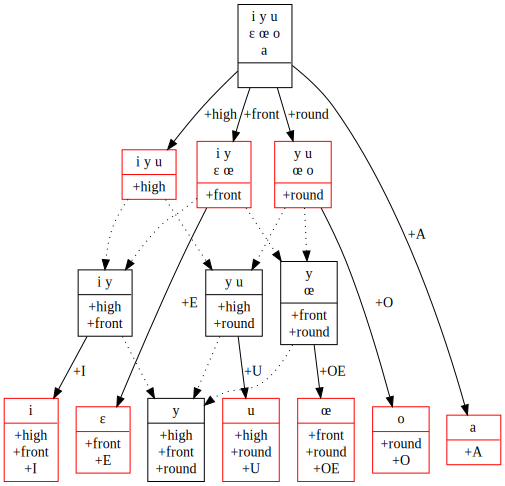
\includegraphics[width=0.6\textwidth]{vowel_inventory_privative.png}
	\caption{Yield of the privative specification algorithm.}
	\label{fig:privative}
\end{figure}

\begin{table}[htb!]
	\centering
	\begin{tabular} {|c||c|c|c|c|c|c|c|c|c|c|}
		\hline
		$\sigma$ & nonlow & front & high & round & a & i & u & e & o & \o \\ \hline
		a & 0 & 0 & 0 & 0 & + & 0 & 0 & 0 & 0 & 0 \\
		i & + & + & + & 0 & 0 & + & 0 & 0 & 0 & 0 \\
		u & + & 0 & + & + & 0 & 0 & + & 0 & 0 & 0 \\
		e & + & + & 0 & 0 & 0 & 0 & 0 & + & 0 & 0 \\
		o & + & 0 & 0 & + & 0 & 0 & 0 & 0 & + & 0 \\
		y & + & + & + & + & 0 & 0 & 0 & 0 & 0 & 0 \\
		\o & + & + & 0 & + & 0 & 0 & 0 & 0 & 0 & + \\
		\hline
	\end{tabular}
	\caption{Featural specification of the vowel system with privative specification.}
	\label{table:privative_vowel_features}
\end{table}

The privative featurization generates a feature system that covers the intersectional closure of the input class system and consists only of privative values. Note that /y/ does not require a \featmat{+y} feature because it is the intersection of the front, high, and round classes.

Any class system can be covered using only privative features, and completely privative systems have been proposed by researchers in the past \cite<e.g.,>{AndersonEwen1987, AveryRice1989, LahiriMarslenWilson1991, Frisch1996}. In these models, `$-$' feature values are unmarked, and thus may be filled in by redundancy rules, or only positive values of features need ever be referred to in the phonology. The privative algorithm generates featurizations consistent with such proposals.

There are valid theoretical reasons to prefer non-privative specifications, however. One argument arises from complement classes, such as ATR vs. RTR vowels. Languages with an ATR/RTR distinction frequently have ATR harmony \cite{ArchangeliPulleyblank1994}. Under privative specification one would need to write one harmony rule for the \featmat{+ATR} feature, and an otherwise identical rule for the \featmat{+RTR} feature. By making the ATR feature binary (i.e., \featmat{$\pm$ATR}), one formally recognizes the sameness of ATR/RTR with respect to the harmony process \cite{Archangeli2011}. In addition, allowing `$-$' feature values will also generally result in feature systems containing fewer features. 

\subsection{Complementary Specification}

Consider the plot of the same vowel system under complementary specification, shown in Fig.~\ref{fig:vowel_inventory_complementary}, and the accompanying feature chart shown in Table~\ref{table:vowel_inventory_complementary}.

% FIGURE 5
\begin{figure}[htb!]
	\centering
	\includegraphics[width=0.6\textwidth]{vowel_inventory_complementary.png}
	\caption{Yield of the complementary specification algorithm.}
	\label{fig:vowel_inventory_complementary}
\end{figure}

\begin{table}[htb!]
	\centering
	\begin{tabular} {|c||c|c|c|c|c|c|c|c|c|}
		\hline
		$\sigma$ & low & front & high & round & i & u & e & o & \o \\ \hline
		a & + & 0 & 0 & 0 & 0 & 0 & 0 & 0 & 0\\
		i & -- & + & + & 0 & + & 0 & 0 & 0 & 0\\
		u & -- & 0 & + & + & 0 & + & 0 & 0 & 0 \\
		e & -- & + & 0 & 0 & 0 & 0 & + & 0 & 0 \\
		o & -- & 0 & 0 & + & 0 & 0 & 0 & + & 0 \\
		y & -- & + & + & + & -- & -- & 0 & 0 & -- \\
		\o & -- & + & 0 & + & 0 & 0 & 0 & 0 & + \\
		\hline
	\end{tabular}
	\caption{Featural specification of the vowel system with complementary specification.}
	\label{table:vowel_inventory_complementary}
\end{table}

Now only nine features are required. The segment /a/, which was \featmat{+nonlow} under the privative algorithm, has instead been featurized as \featmat{--low} here. This is because the low and non-low classes are complements with respect to their parent ($\Sigma$), and both are present in the input. Contrastive \featmat{low} is doing the work of privative \featmat{low} and privative \featmat{nonlow} together, so there is no need for a contrastive \featmat{nonlow} feature.

An additional point of note is that /y/ is assigned the feature/value pairs \featmat{--\textipa{i}}, \featmat{--u}, and \featmat{--\textipa{\o}}, and hence these features are now ternary. This occurs because /y/ is a complement to the classes with single parents that motivate the addition of these features.

In general, the requirements for receiving a \featmat{$-f$} value are not as strict as receiving a \featmat{$+f$} value: \featmat{$-f$} classes may have more than one parent (as \{y\} does here). In addition, they do not necessarily need to be siblings of the class motivating the addition of the new feature, although in Fig.~\ref{fig:vowel_inventory_complementary} they happen to be. Restricting the assignment of \featmat{$-f$} values in the same way as \featmat{$+f$} values introduces complications for other types of featurization presented here, such as the full specification algorithm. Note that the remaining features (\featmat{front}, \featmat{high}, \featmat{round}, \featmat{\textipa{e}}, \featmat{o}) are still privative, because their respective complements are not present in the input. 

The type of featurization generated by the complementary specification algorithm is consistent with many contemporary feature systems, where some features are privative (e.g., \featmat{LABIAL}), some are binary (e.g., \featmat{son}), and some are ternary (e.g., \featmat{back}. This most closely resembles systems that assume what \citeA{Archangeli1988} calls \textit{contrastive specification}: feature/value pairs are assigned only to the subset of segments where the feature is distinctive. 

Consistent with much work on underspecification \cite<e.g.,>{Archangeli1984, ArchangeliPulleyblank1989, ArchangeliPulleyblank1994}, this model predicts that underspecification may vary across languages. The typological regularities that have led researchers to propose certain features as being inherently underspecified, such as the place features \featmat{LABIAL}, \featmat{CORONAL}, and \featmat{DORSAL} \cite<e.g.,>{Sagey1986} are considered to be consequences of the system that identifies classes in a language, rather than a restriction on the kinds of contrasts feature systems can encode. This model is also incompatible with theories where markedness plays some role in determining featural specification \cite<see section 2.1.3 in >[ and references therein]{Archangeli1988}, since there is no notion  of markedness encoded in the model.

The particular featurization derived here using contrastive specification does not seem linguistically plausible, but as the next section will show, this is largely a consequence of the particular input classes chosen. See Section~\ref{sec:feature_theory} for an example of a more realistic featurization derived using contrastive specification.

\subsection{Conservational properties of featurizations}

One point to observe is that the privative specification and complementary specification algorithms are \textit{maximally conservative}. What we mean by this is that the resulting feature system generates the smallest class system that covers $C$. As the Intersectional Closure Covering Theorem showed, any featurization which covers $C$ will cover $C_\cap$. This means that any classes which are the intersection of input classes, but which were not themselves in the input, will be accessible to the output feature system. But the privative and complementary specification algorithms will not make it possible to refer to any other classes outside the intersectional closure. For example, the vowel system here contains a \featmat{+front} class and a \featmat{+round} class, and it necessarily generates a \featmattwo{+front}{+round} class. However, it does not infer the existence of a \featmat{--round} class based on the existence of the \featmat{+round} class.

It is easy to show that one can sometimes achieve a more efficient feature system by adding classes to the system. For example, the privative featurization of the vowel system contains ten features, and the complementary specification featurization contains nine. If we change the input to consist of the classes shown in Table~\ref{table:vowels2}, however, the privative specification algorithm returns a featurization with eight features, and complementary specification returns one with only four features. The privative system requires two fewer features because the addition of the mid, back, and unround classes requires an additional three features (\featmat{back}, \featmat{unround}, and \featmat{mid}), but allows us to remove five singleton features (all except \featmat{a}), since the corresponding singleton classes can now be generated by the intersection of larger classes. This is also true for the contrastive system, which in addition can remove the \featmat{mid}, \featmat{back}, \featmat{unround}, and \featmat{a} features, since they fall into a complementary relationship with the \featmat{+high}, \featmat{+front}, \featmat{+round}, and \featmat{+nonlow} classes respectively, and can be assigned `$-$' values for those features. Crucially, these featurizations cover the original class system shown in Fig.~\ref{fig:vowel_inventory}. Thus, they use fewer features while generating a richer class system.

\begin{table}[h]
	\centering
	\begin{tabular} {|l|l|}
		\hline
		\textit{alphabet} & \{\textipa{a}, \textipa{i}, \textipa{u}, \textipa{e},  \textipa{o}, \textipa{y}, \textipa{\o}\} \\
		\hline
		\textit{non-low} & \{\textipa{i}, \textipa{u}, \textipa{e},  \textipa{o}, \textipa{y}, \textipa{\o}\} \\
		\hline
		\textit{high} & \{\textipa{i}, \textipa{u}, \textipa{y}\} \\
		\hline
		\textit{\textbf{mid}} & \textbf{\{e, o, \o\}} \\
		\hline
		\textit{front} & \{\textipa{i}, \textipa{e}, \textipa{y}, \textipa{\o}\} \\
		\hline
		\textit{\textbf{back}} & \textbf{\{u, o\}} \\
		\hline
		\textit{round} & \{\textipa{u}, \textipa{o}, \textipa{y}, \textipa{\o}\} \\
		\hline
		\textit{\textbf{unround}} & \textbf{\{i, e\}} \\
		\hline
		\textit{singletons} & \{\textipa{a}\}, \{\textipa{i}\}, \{\textipa{u}\}, \{\textipa{e}\}, \{\textipa{o}\}, \{\textipa{y}\}, \{\textipa{\o}\} \\
		\hline
	\end{tabular}
	\caption{Vowel inventory with extra classes (bolded)}
	\label{table:vowels2}
\end{table}

This example is presented to make two points. First, the relationship between classes in the input and the specification algorithm is not monotone. In general, adding features to a system will make more classes accessible -- but in this example, a smaller number of features covers a larger class system. Thus, the minimal number of features needed to cover $C$ is not predictable from a simple property, such as the total number of classes in $C$. More precisely, the privative specification algorithm is an upper bound on the  number of features needed to cover a class system (namely, the number of classes in the intersectional closure with a single parent). We return to the issue of feature efficiency and expressiveness in Section \ref{sec:discussion}. 

In the meantime, we turn to the second point this example makes -- adding the `right' classes to the input enables a more economical feature system. This is exactly what the inferential complementary and full specification algorithms do, differing only in which classes they add.

\subsection{Inferential complementary specification}

Fig.~\ref{fig:vowel_inventory_ic} illustrates the featural plot of the IC specification algorithm on the vowel system, with the corresponding feature chart shown in Table~\ref{table:vowel_inventory_ic} (the topological plot is shown in Appendix~\ref{app:topological}). Now the complement classes with respect to their parent of the round, high, and front classes have been added, resulting in a more efficient and expressive featurization containing only binary or ternary features. Only /a/ has any unspecified values, since it is a child only of $\Sigma$. In fact, this algorithm infers the same classes that we added in the vowel system in Table~\ref{table:vowels2} above.

% FIGURE 6
\begin{figure}[htb!]
	\centering
	\includegraphics[width=0.75\textwidth]{vowel_inventory_ic_FEATURAL.png}
	\caption{Class system and featurization yielded by IC specification. Classes explicitly added by the algorithm are indicated with dashed boxes. Classes added due to the addition of these classes to the intersectional closure are not highlighted.}
	\label{fig:vowel_inventory_ic}
\end{figure}

\begin{table}[htb!]
	\centering
	\begin{tabular} {|c||c|c|c|c|}
		\hline
		$\sigma$ & low & front & high & round \\ \hline
		a & + & 0 & 0 & 0 \\
		i & -- & + & + & -- \\
		u & -- & -- & + & + \\
		e & -- & + & -- & -- \\
		o & -- & -- & -- & + \\
		y & -- & + & + & + \\
		\o & -- & + & -- & + \\
		\hline
	\end{tabular}
	\caption{Featural specification of the vowel system with IC specification.}
	\label{table:vowel_inventory_ic}
\end{table}

Note that while the class systems for the privative and contrastive specifications shown in Figs.~\ref{fig:privative} and~\ref{fig:vowel_inventory_complementary} are identical to the input and to each other, the derived class system in Fig.~\ref{fig:vowel_inventory_ic} is substantially larger. In particular, despite only three classes being explicitly added by the algorithm (the \featmat{--round}, \featmat{--high}, and \featmat{--front} classes), the resulting class system contains a total of 20 classes, while the input contained only 15. The additional two classes are the result of intersectional closure generating \featmattwo{--high}{+round} and \featmattwo{--high}{+front} classes.

The addition of these classes produces a more efficient featurization that covers the same classes as the complementary algorithm, at the cost of altering the original class system. Thus this featurization reflects a model of feature learning that differs in an important way from the previous two algorithms.

We assume that the input classes for these algorithms have been motivated by the phonetics and phonology of the language. The privative and complementary algorithms differ primarily on theoretical grounds: do we wish to allow `$-$' feature values, or not? The difference between these algorithms and the IC and full specification algorithms is somewhat more substantial, however: the latter assume that learners are capable of some degree of generalization, inferring new classes based on the structure of existing classes, rather than on explicit phonetic or phonological evidence. They differ in terms of how the new classes are defined. For the IC algorithm, the learner infers the existence of complement classes with respect to the parent of classes that only have a single parent, if these complements are not present in the input. The full featurization algorithm infers the existence of complement classes with respect to $\Sigma$, and in doing so eliminates all underspecification from the resulting feature system.

\subsection{Full specification}

The featural plot of the full specification algorithm on the vowel system is shown in Fig.~\ref{fig:vowel_inventory_full}, and the corresponding feature chart is shown in Table~\ref{table:vowel_inventory_full} (the topological plot is shown in Appendix~\ref{app:topological}).

\begin{figure}[htb!]
	\centering
	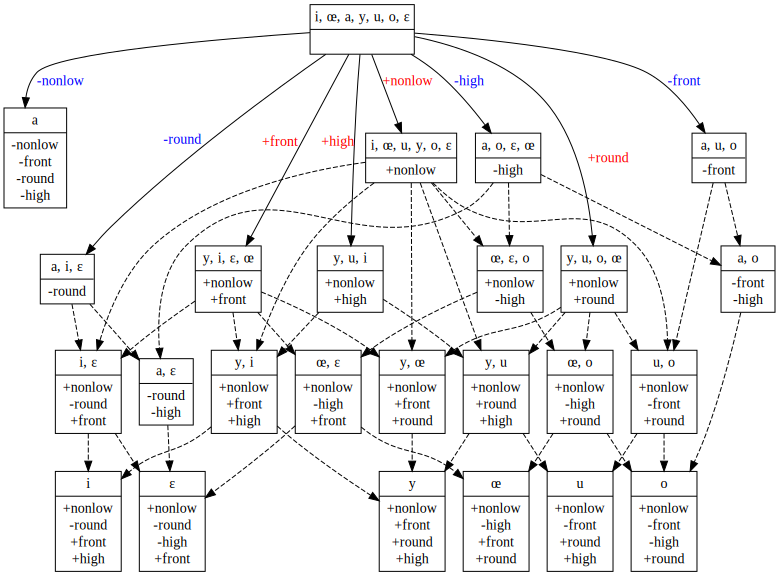
\includegraphics[width=0.9\textwidth]{vowel_inventory_full_FEATURAL.png}
	\caption{Class system and featurization yielded by full specification.  Classes explicitly added by the algorithm are indicated with dashed boxes. Classes added due to the addition of these classes to the intersectional closure are not highlighted.}
	\label{fig:vowel_inventory_full}
\end{figure}

\begin{table}[htb!]
	\centering
	\begin{tabular} {|c||c|c|c|c|}
		\hline
		$\sigma$ & low & front & high & round \\ \hline
		a & + & -- & -- & -- \\
		i & -- & + & + & -- \\
		u & -- & -- & + & + \\
		e & -- & + & -- & -- \\
		o & -- & -- & -- & + \\
		y & -- & + & + & + \\
		\o & -- & + & -- & + \\
		\hline
	\end{tabular}
	\caption{Featural specification of the vowel system with full specification.}
	\label{table:vowel_inventory_full}
\end{table}

The number of features in the full featurization is the same as the IC featurization, but now /a/ is fully specified for all features, and several new classes have been introduced as a consequence, significantly altering the overall structure of the class system.

As in the IC algorithm, only three new classes are explicitly added to the class system: the \featmat{--round}, \featmat{--high}, and \featmat{--front} classes. However, the resulting class system now contains 25 classes rather than 20. This is a consequence of these new classes containing the segment /a/, which greatly increases the number of classes accessible in the intersectional closure. Because /a/ is now specified for all features, the classes specified by the featural descriptors  \featmat{--front}, \featmat{--high}, \featmat{--round}, \featmattwo{--front}{--high} and \featmattwo{--round}{--high} now contain /a/. The same classes that were characterized by these featural descriptors under the IC featurization can only be picked out by adding \featmat{--low} to each of these descriptors, resulting in the additional five classes we see.

A key way in which full specification differs from IC specification is that no underspecification can occur whatsoever. This is due to the domain over which new classes are created: IC specification creates new classes with respect to the parent of the class motivating the new features, while full specification creates them with respect to the entire alphabet.

For example, if a single feature \featmat{+nasal} is used to pick out nasal segments, then the feature system will also generate the class \featmat{--nasal} consisting of all non-nasal segments. According to our understanding of nasal typology, this is probably not the desired behavior for the nasal feature \cite<e.g.,>{Trigo1993}.\footnote{Though see, e.g., \citeA{Padgett2002} for an analysis that relies on \featmat{--nasal} specification.} However, it is possible to avoid generating a \featmat{--nasal} class by ensuring that the nasals are generated as the union of pre-existing features, rather than needing their own feature. For example, if \featmat{--continuant} picks out the nasals and oral stops, while \featmat{+sonorant} picks out vowels, glides, liquids, and nasals, then the nasal class is picked out by \featmattwo{--continuant}{+sonorant}. Therefore, the set of all non-nasals will not be generated as a complement class because the \featmat{+nasal} feature is not generated at all. A desirable property of this solution is that the following classes fall out: continuant non-sonorants (fricatives), continuant sonorants (approximants), and non-continuant non-sonorants (stops and affricates). Less desirably, this solution fails to transparently represent nasal spreading processes; for example, vowel nasalization cannot be described as continuancy or sonorancy assimilation. Thus, the cross-linguistic behavior and learnability of classes like \featmat{--nasal} has the potential to inform feature theory. We take up this and other issues in Section \ref{sec:discussion}.

\FloatBarrier
\section{Discussion}
\label{sec:discussion}

In this paper, we have described a number of algorithms which assign a featurization to a set of classes, such that every class in the input can be picked out by a featural descriptor. We gave several variants of the algorithm, differing in the types of features they assign and how conservative they are with respect to the input. The most conservative algorithm assigns a privative specification, i.e., feature functions which only pick out positively specified elements. Complementary specification is achieved with the same algorithm, except that a negative specification is assigned just in case the complement of a class with respect to its parent class is in the input. Inferential complementary specification is similar, except that a negative specification is assigned even if the complement with respect to the parent was not in the input. Full specification is similar to IC specification, except the complement is taken with respect to the entire segmental alphabet. In this section, we discuss some outstanding issues, such as feature efficiency and expressiveness, and how the current work bears on feature theory.

\subsection{Feature efficiency and expressiveness}

Here we present examples which further illustrate the expressiveness of class systems.

Let $C = \{ \{\sigma\} \, | \, \sigma \in \Sigma \}$; that is, the input consists of all and only the singleton sets. For convenience, we will refer to this as the \textit{singleton input}. Privative specification will yield a featurization with $n$ features, where $n$ is the cardinality of $\Sigma$. This is because each segment gets its own feature, since the only parent of each segment is $\Sigma$. This featurization will generate only the classes in the input (and $\Sigma$, and $\varnothing$).

The opposite extreme is obtained by the \textit{singleton complement} input -- where the input consists not of all singleton sets, but the complement of each singleton set:  $C = \{ \Sigma \setminus \{\sigma\} \, | \, \sigma \in \Sigma \}$. It is possible to show that when the privative specification algorithm is given this input, it generates the full powerset of $\Sigma$ -- every possible subset gets a unique combination of features. This follows from the fact that any set can be defined by listing the features for the segments not contained in it. Thus, privative specification is still compatible with a maximally expressive system.

The powerset of $\Sigma$ is also generated by running the full specification algorithm on the singleton input. Thus, there are cases where a more conservative algorithm yields the same class system as a less conservative algorithm (albeit with a different number of features). In fact, it is generally true that the more conservative algorithms can achieve the same level of expressiveness as any less conservative algorithm, by virtue of including the relevant complement classes in the input. For example, if all complement classes with respect to $\Sigma$ are included, the privative specification algorithm yields the same class system as the full specification one does, although with twice the number of features (the singleton complement input discussed above is a special case of this). Moreover, complementary specification, IC specification, and full specification all yield the same featurization (as well as the same class system) if every relevant complement class is included. In short, the algorithms can yield radically different class systems depending on their input -- but all can be made highly expressive by tailoring the input appropriately.

\subsection{Relation to feature theory}
\label{sec:feature_theory}

As the examples in the preceding section illustrate, the most conservative algorithms (privative and complementary specification) are able to yield class systems that are as expressive as the less conservative algorithms. However, the converse is not true. For example, full specification cannot yield a class system as unexpressive as the singleton input does under privative specification. So which algorithm best reflects our knowledge of feature systems? One principle is that a feature system is good to the extent that learned features render the grammar simpler and/or more insightful. For example, the use of `$+$' and `$-$' values yields insight if both values behave in the same way with respect to a harmony or assimilation process.

Although there are exceptions, most commonly employed feature systems generally recognize the following cases: (a) treat certain features as binary: e.g., all segments are either \featmat{+son} or \featmat{--son}; (b) treat certain features as privative: e.g., nasals are \featmat{+nasal} and all others are \featmat{0nasal}; (c) treat most features as ternary: e.g., all vowels are \featmat{+ATR} or \featmat{--ATR}, but consonants are simply \featmat{0ATR}.

Out of the algorithms we have discussed here, only the complementary algorithms are capable of yielding a featurization which creates all three feature types. The distinction between complementary and inferential complementary featurizations depends on whether complements of input classes with respect to their parents must also be in the input (which perhaps corresponds to phonological activeness) or can be defined implicitly. This is an issue that can be resolved empirically.

The complementary algorithm creates those three types of feature functions under the following conditions. Binary features are generated when a class $X$ and its complement $\Sigma \setminus X$ are both in the input. Privative features are generated when a class $X$ is in the input, but no complement (with respect to any ancestor, including its parent, $\Sigma$, and any intervening classes) is. Ternary features are generated when a class $X$ is in the input, and its complement $\overline{X}$ with respect to its parent other than $\Sigma$ is in the input.

For reasons of space, we do not prove that those are the correct conditions. Instead, we present an example which generates privative, binary, and ternary features. Let $C$ include the classes in Table~\ref{table:big_features}.

\begin{table}[h]
	\centering
	\begin{tabular} {|l|l|}
		\hline
		\textit{alphabet } & \{a, i, u, l, r, m, n, \textipa{N}, p, t, k, b, d, \textipa{g}\} \\
		\hline
		\textit{consonants} & \{l, r, m, n, \textipa{N}, p, t, k, b, d, \textipa{g}\} \\
		\hline
		\textit{sonorants} & \{a, i, u, l, r, m, n, \textipa{N}\} \\
		\hline
		\textit{obstruents} & \{p, t, k, b, d, \textipa{g}\} \\
		\hline
		\textit{coronal} & \{n, l, r, t, d\} \\
		\hline
		\textit{vowels} & \{a, i, u\} \\
		\hline
		\textit{nasals} & \{m, n, \textipa{N}\} \\
		\hline
		\textit{voiceless} & \{p, t, k\} \\
		\hline
		\textit{voiced} & \{b, d, \textipa{g}\} \\
		\hline
		\textit{labial} & \{m, p, b\} \\
		\hline
		\textit{dorsal} & \{\textipa{N}, k, \textipa{g}\} \\
		\hline
		\textit{liquids} & \{l, r\} \\
		\hline
		\textit{lateral} & \{l\} \\
		\hline
		\textit{rhotic} & \{r\} \\
		\hline
	\end{tabular}
	\caption{A large class system}
	\label{table:big_features}
\end{table}
We omit most of the singleton sets for reasons of exposition, although many are derived by intersectional closure. The class system that results from running the complementary algorithm on this input is shown in Fig.~\ref{fig:big_alphabet}. The features \featmat{cons} and \featmat{son} are binary because each one partitions $\Sigma$. The features \featmat{LAB}, \featmat{COR}, \featmat{DOR}, \featmat{nas} and \featmat{liquid} are privative, because their complement (with respect to every ancestor) is not included in the input. The remaining features \featmat{voice} and \featmat{lat} are ternary, because their complements (with respect to the parent, which is not $\Sigma$) are included in the input. We invite the reader to determine what happens to the \featmat{voice} feature if the input includes the class of all phonetically voiced segments (i.e., $\Sigma \setminus \text{\{p, t, k\}}$).

\begin{figure}[htb!]
  \centering
  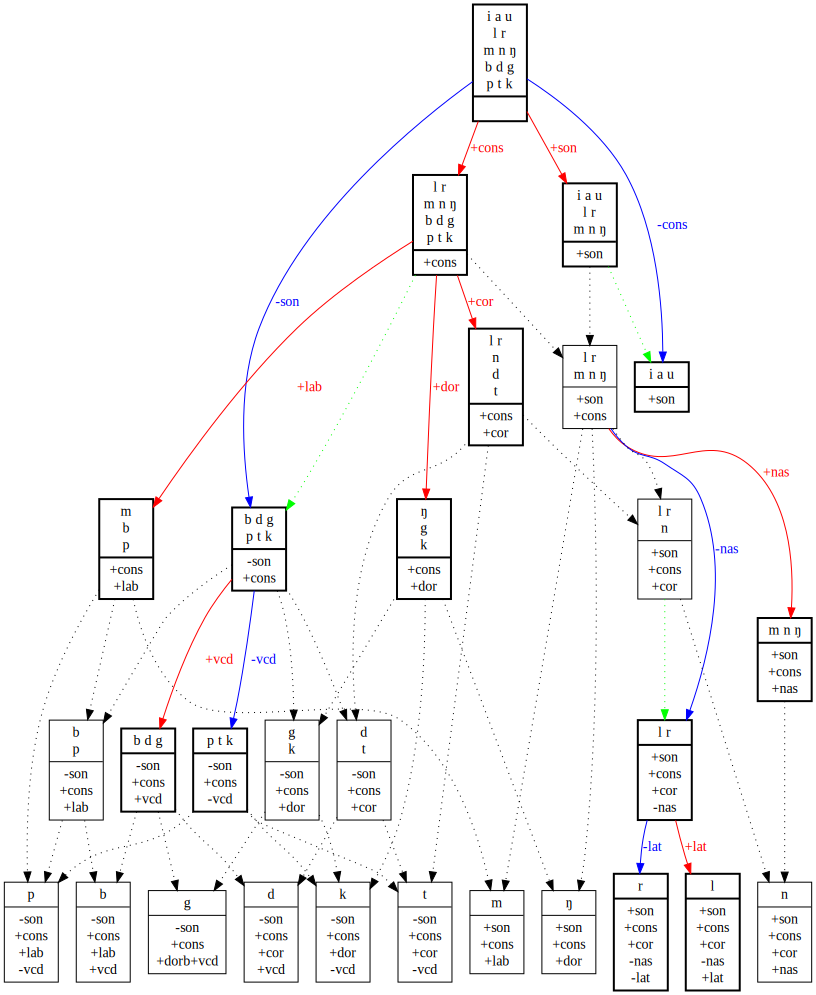
\includegraphics[width=\textwidth]{biggun.png}
  \caption{The output of complementary specification on a large class system. }
  \label{fig:big_alphabet}
\end{figure}

It is our hope that the algorithms described in this paper might be used in generating explicitly testable empirical hypotheses on learning phonological features. Varying the input classes and the featurization method generates different predictions about the available phonological classes in a language. This is particularly true in the cases of the IC and full specification algorithms, where new classes are inferred based on the relationships between classes in the input. These featurizations provide a starting point for hypotheses that are testable in phonological experiments. For example, are speakers able to infer the existence of productive phonological classes for which the only evidence in the input is that the complement (with respect to some ancestor) behaves productively? 

Because these algorithms generate underspecification as a function of the relationship between the input classes, it may be expected to vary cross-linguistically. In addition, the model of feature learning requires that notions of markedness not be a determining factor in underspecification. The appropriate application of underspecification has been somewhat controversial in the past \cite<e.g.,>{Steriade1995}. A contribution of this paper is that it provides a completely deterministic method for generating underspecification, depending only on the input classes and the featurization method used. This is perhaps similar to hierarchical decision-tree systems \cite<e.g.,>{Dresher2003, Hall2007}, except that in such models, the hierarchical ordering of features must be specified by the analyst, while here it falls out naturally from the relations between the input classes. An unambiguous method for determining underspecification is doubtless of value to the field, and we leave as a question for future research how closely the methods described here line up with past analyses, and whether the predictions they make are borne out empirically.

We have not discussed the possibility of applying `$-$' feature values to complements with respect to an ancestor other than the parent or $\Sigma$. This bears directly on where underspecification should occur. For example, we may want to specify every coronal obstruent as either \featmat{+strident} or \featmat{--strident}, and all non-coronals as \featmat{0strident}. It is less clear, though, whether coronal sonorants should be specified as \featmat{--strident} or \featmat{0strident}. Defining the \featmat{--strident} class as the complement of the \featmat{+strident} class with respect to just the set of coronal obstruents will result in coronal sonorants being unspecified for \featmat{strident}, while defining it as the complement with respect to the full class of coronals will result in coronal sonorants being \featmat{--strident}. We do not put forth a concrete proposal for how one might choose which ancestor to use for complementation, but a possible strategy would be to consider the complement with respect to every ancestor of the target class, and choose the one that results in the most efficient feature system (by some criterion), or that avoids implausible features (perhaps based on phonetic criteria). We leave this as a possible area for future research informed by empirical phonological evidence.

Finally, it is worth touching briefly upon the challenges for underspecification theory posed by Richness of the Base \cite{PrinceSmolensky1993}. This stipulates that there are no constraints on the input, and so a grammar must be able to deal sensibly with both fully specified and underspecified forms. This rules out analyses that rely on certain segments being underspecified in the input, but underspecification is still permitted, and important for other reasons. For example, if phonological constraints are learned from positive input data \cite<e.g.,>{HayesWilson2008}, underspecified features serve an important role in constraining the generalizations the learner may make by limiting what the phonological grammar can reference. We also note that language-specific features complicate the handling of non-native input forms. We follow \citeA{Hall2007} in suggesting that the answer for this lies in a better understanding of how speakers map acoustic input onto the phonological representations of their language.

\FloatBarrier
\section{Conclusion}
\label{sec:conclusion}

This paper provides a detailed formalization of the properties of phonological feature systems and describes algorithms for efficiently calculating various types of featurizations of a set of input classes. An implementation of these algorithms is available for use in further research. This work provides a stronger formal grounding for the study of phonological features, may serve as a useful component in computational models of feature learning, and makes concrete predictions about the sources of phonological underspecification and how learners might generalize across classes. We hope that these predictions will provide useful, testable empirical hypotheses for future experimental phonological research.

\appendix

\section{Calculating the intersectional closure}
\label{app:closure}
The following algorithm yields the intersectional closure of a class system $(C, \Sigma)$. It bears a close resemblance to Dijkstra's shortest-paths algorithm \cite{Dijkstra1959}. Names used in the pseudocode below are defined in Table~\ref{table:algorithm_definitions}.
\noindent \begin{algorithmic}
	\singlespacing
	\ENSURE $C'$ is the intersectional closure of the input class system ($C, \Sigma)$
	\STATE
	\STATE $C' \leftarrow \{ \Sigma \} $
	\STATE $Q \leftarrow C$
	\STATE
	\WHILE{$Q \neq \varnothing$}
	\STATE $X \leftarrow \textsc{dequeue}(Q)$
	\IF{\NOT $X \in C'$}
	\FOR{$Y \in C'$}
	\STATE $\textsc{enqueue}(Q, X \cap Y)$
	\ENDFOR
	\STATE $C' \leftarrow C' \cup \{ X \}$
	\ENDIF
	\ENDWHILE
\end{algorithmic}
\doublespacing

\noindent The proof of the algorithm's soundness goes by induction. First, we show that every class which can be generated by the intersection of $0$ classes ($\Sigma$) or 1 class from $C$ (i.e., $C$ itself) belongs to $C'$. Next, we prove the induction step: if every class that can be generated by the intersection of $n$ classes from $C$ is in $C'$, then every class that can be generated by the intersection of $n+1$ classes from $C$ is in $C'$.

$C'$ is initialized to contain $\Sigma$. Moreover, $Q$ is initialized to contain every class in $C$. Each of these must be transferred to the intersectional closure because they do not belong to it already (dequeued from $Q$, and appended to $C'$). This demonstrates that every intersection of 0 classes ($\Sigma$) and 1 class from $C$ (namely, $C$ itself) belongs to $C'$.

Now, suppose that the algorithm has guaranteed that every intersection of $n$ classes from $C$ is in $C'$. If there exists a $Y \in C'$ which can be written as the intersection of $n+1$ classes, i.e., $Y = X_1 \cap X_2 \cap \ldots \cap X_{n+1} = Y' \cap X_{n+1}$ where $Y' = X_1 \cap X_2 \cap \ldots \cap X_n$. Since every intersection of $n$ classes is in $C'$, $Y'$ must be in $C'$. Now, regardless of whether $X_{n+1}$ was transferred from $Q$ to $C'$ before or after $Y'$ was, there was some point at which one was in $Q$ and the other in $C'$. When the \textbf{for} loop dequeued the one in $Q$, it added the intersection of this one with all others in $C'$ -- i.e., $Y' \cap X_{n+1}$. Either this class was already in $C'$, or else it was not; and in the latter case, it was transferred. Thus, all sets generated by the intersection of $n+1$ classes from $C$ are in $C'$. $\square$


\section{The breadth-first algorithm for adding complement classes}
\label{app:complements}

The inferential complementary (IC) and full featurization algorithms add classes to $C_\cap$ during their execution. In this section, we provide descriptions of the \textsc{AddComplements} and \textsc{AddComplementsFull} algorithms introduced in Sections \ref{sec:contrastive} and \ref{sec:full}. We then motivate the use of breadth-first traversal using examples where traversing the classes in an arbitrary order produces spurious features, and discuss considerations on the order in which siblings are processed.

\subsection{The algorithms}

The algorithms for adding complement classes traverse $C_\cap$ and, for classes with a single parent, add their complement with respect to their parent (IC specification) or $\Sigma$ (full specification) to the class system. In order to avoid specifying spurious features, $C_\cap$ must be traversed in \textit{breadth-first order}: that is, processing all the siblings of a class before processing any of its children. We provide some examples where this results in more efficient feature systems in Appendix~\ref{app:bfs}. We conjecture that breadth-first traversal will always produce identical or smaller feature systems than traversal in an arbitrary order, but do not provide formal proofs here. In addition, siblings are processed simultaneously, and all their generated complements (if any) are added to the class system simultaneously. The motivation for this is discussed in Appendix~\ref{app:siblings}.

Below is the algorithm for \textsc{AddComplements}:
\noindent \begin{algorithmic}
	\singlespacing
	\REQUIRE $C_\cap$ is the intersectional closure of input class system $(C, \Sigma)$
	\STATE
	\STATE $Q \leftarrow \{\Sigma\}$
	\STATE
	\WHILE{$Q \neq \varnothing$}
	\STATE $X \leftarrow \textsc{dequeue}(Q)$
	\STATE $\textsc{ChildClasses} \leftarrow \textsc{children}_C(X)$
	\STATE $\textsc{ChildComplements} \leftarrow \varnothing$
	\WHILE{$\textsc{ChildClasses} \neq \varnothing$}
	\STATE $Y \leftarrow \textsc{dequeue}(\textsc{ChildClasses})$
	\IF{$| \textsc{parents}_C(Y) | = 1$}
	\STATE $\overline{Y} \leftarrow X \setminus Y$
	\STATE $\textsc{ChildComplements} \leftarrow \textsc{ChildComplements} \cup \overline{Y}$
	\ENDIF
	\ENDWHILE
	\STATE $C_\cap \leftarrow \textsc{IntersectionalClosure}(C_\cap, Q' = \textsc{ChildComplements})$
	\STATE $\textsc{NewChildren} \leftarrow \textsc{children}_C(X)$
	\STATE $Q \leftarrow Q \cup \textsc{NewChildren}$
	\ENDWHILE
\end{algorithmic}
\doublespacing

\noindent \textsc{AddComplementsFull} is identical, except the complement is taken with respect to $\Sigma$ rather than the parent (i.e., the line $\overline{c} \leftarrow p \setminus c$ is replaced with $\overline{c} \leftarrow \Sigma \setminus c$).

\subsection{Breadth-first vs. arbitrary traversal}
\label{app:bfs}

A new feature only needs to be added when a class has a single parent. The IC and full specification algorithms add the complement with respect to the parent and the alphabet, respectively. These new classes alter the class structure, meaning that a class that has a single parent at one point may have two parents after a class is added. Thus redundant classes and features may be added if a class with a single parent is processed before another class whose complement would become a parent of the first class.

\begin{figure}[htb!]
	\centering
	\includegraphics[width=0.2\textwidth]{bfs1.png}
	\caption{A simple class system.}
	\label{fig:bfs1}
\end{figure}

Consider the input classes shown in Fig.~\ref{fig:bfs1}, and suppose we are processing them using full specification (i.e., adding complement classes with respect to $\Sigma$). If \{c, e, f\} is processed before \{a, b\}, its complement with respect to $\Sigma$, \{a, b, d\} will be added to the class system. When \{a, b\} is processed later, its complement with respect to $\Sigma$, \{c, d, e, f\} is added to the class system, and becomes an additional parent to \{c, e, f\}. This results in the feature system shown on the left side of Fig.~\ref{fig:bfsfeats}. Note that the only purpose of F3 is to differentiate the newly added class \{a, b, d\}, whose presence is unmotivated since \{c, e, f\}, the class which generated it, ends up having two parents.

\begin{figure}[htb!]
	\centering
	\subfloat{{\includegraphics[width=0.3\textwidth]{bfs1_feats.png}}}
	\qquad
	\subfloat{{\includegraphics[width=0.3\textwidth]{bfs2_feats.png}}}
	\caption{The classes generated after running \textsc{AddComplementsFull} if classes are processed in an arbitrary order (left) and in breadth-first order (right).}
	\label{fig:bfsfeats}
\end{figure}

%\begin{figure}[htb!]
%	\centering
%	\includegraphics[width=0.4\textwidth]{bfs1_feats.png}
%	\caption{The classes generated after running \textsc{AddComplementsFull} if classes are processed in an arbitrary order.}
%	\label{fig:bfs1feats}
%\end{figure}

Now consider the same input, but suppose that we process \{a, b\} before \{c, e, f\} (i.e., in breadth-first order). Processing \{a, b\} adds its complement with respect to $\Sigma$, \{c, d, e, f\}, which becomes the second parent to \{c, e, f\}. Now when \{c, e, f\} is processed, its complement with respect to $\Sigma$ is not added because it does not have only a single parent. This results in the feature system shown on the right side of Fig.~\ref{fig:bfsfeats}.

%\begin{figure}[htb!]
%	\centering
%	\includegraphics[width=0.4\textwidth]{bfs2_feats.png}
%	\caption{The classes generated after running \textsc{AddComplementsFull} if classes are processed in breadth-first order.}
%	\label{fig:bfs2feats}
%\end{figure}

Note that the breadth-first feature system is exactly as expressive as the arbitrary system, with the exception of the unmotivated class \{a, b, d\}. Both cover the original input. A similar example can be generated for the IC case.

Thus using breadth-first traversal produces a smaller featurization system that differs only in its ability to generate unmotivated classes. We conjecture that using breadth-first traversal guarantees that when a class is processed, all of its parents that will be added to the input by the end of the algorithm will have already been added, but we leave the proof as a question for future research.

\subsection{Considerations on the ordering of siblings}
\label{app:siblings}

Although breadth-first traversal gives us a rough guide for how to process classes, it does not completely determine the order. The question of the order in which siblings should be processed is still unanswered. Here, too, ordering proves to be important for the resulting class system. Consider the input shown in Fig.~\ref{fig:siblinginput}, and suppose this time that we are running the IC specification algorithm.

\begin{figure}[htb!]
	\centering
	\includegraphics[width=0.25\textwidth]{sibling_input.png}
	\caption{A simple class system.}
	\label{fig:siblinginput}
\end{figure}

Suppose we process the class \{b\} before either of the other classes. This will result in the complement of \{b\} with respect to $\Sigma$, \{d, g\}, being added to the class system. This is shown on the left side of Fig.~\ref{fig:siblingoutput}.

\begin{figure}[h]
	\centering
	\subfloat{{\includegraphics[width=0.25\textwidth]{sibling_output1.png}}}
	\qquad
	\subfloat{{\includegraphics[width=0.25\textwidth]{sibling_output2.png}}}
	\caption{The resulting feature systems when siblings are processed sequentially (left) and simultaneously (right) using the IC specification algorithm.}
	\label{fig:siblingoutput}
\end{figure}

%\begin{figure}[htb!]
%	\centering
%	\includegraphics[width=0.3\textwidth]{sibling_output1.png}
%	\caption{The resulting feature system when siblings are processed sequentially using the contrastive specification algorithm.}
%	\label{fig:siblingoutput1}
%\end{figure}

This is troubling, however, because it predicts that the class \{d, g\} should be available in the phonology, while the similar classes \{b, g\} and \{b, d\} should not. This prediction is unmotivated by the class structure, and occurs in some form regardless of which class is processed first.

%\begin{figure}[htb!]
%	\centering
%	\includegraphics[width=0.3\textwidth]{sibling_output2.png}
%	\caption{The resulting feature system when siblings are processed simultaneously.}
%	\label{fig:siblingoutput2}
%\end{figure}

In light of this observation, and given the lack of an obvious principled way to choose which class should be processed first, we process siblings \textit{simultaneously}: that is, the complements of \textit{all} siblings are calculated, and added to the class system at the same time. In this case, the resulting class system is shown on the right side of Fig.~\ref{fig:siblingoutput}.

This feature system is less efficient, in the sense that it requires more features, but the overall structure is the one best motivated by the input classes. If the simpler structure is indeed the desired one, the class \{d, g\} can simply be added to the input.

When the full specification algorithm is run on the input in Fig.~\ref{fig:siblinginput} with sequential processing, a similarly arbitrary class structure is generated, although in this case it involves two of the three possible two-segment subclasses rather than only one.

\subsection{Topological plots}
\label{app:topological}

These are the topological plots of the output the IC and full specification algorithms on the vowel system. The parent/child relationship is maintained in the graph, but featural siblings (i.e., +/- pairs) are not necessarily plotted at the same level.

\begin{figure}[htb!]
	\centering
	\includegraphics[width=0.65\textwidth]{vowel_inventory_ic_TOPOLOGICAL.png}
	\caption{The topological plot of the output of the IC specification algorithm.}
	\label{fig:vowel_inventory_ic_topological}
\end{figure}

\begin{figure}[htb!]
\centering
\includegraphics[width=0.7\textwidth]{vowel_inventory_full_TOPOLOGICAL.png}
\caption{The topological plot of the output of the full specification algorithm.}
\label{fig:vowelfulltopological}
\end{figure}

\bibliography{mybib}
\bibliographystyle{apacite}

%\theendnotes

\end{document}
